\documentclass[]{IEEEtran}

\title{REST APIs Development and Performance Evaluation on the ICELab Kubernetes-based Architecture}
\author{Fabio Chiarani - VR445566}

\usepackage{graphicx}
\usepackage[british]{babel}
\usepackage{multicol}

\usepackage{tikz}

\usepackage{pgf-umlsd}
\usetikzlibrary{arrows,automata, positioning}
\usepackage[latin1]{inputenc}


\usepackage{forest}
\usepackage{xcolor}
\usepackage{listings}
\usepackage{booktabs}
\usepackage{hyperref}
\usepackage{pgfplots}
\usepackage{rotating}
\usepackage{tabularx}
\usepackage{graphicx}
\graphicspath{ {./fig/} }
\lstset {language = C,
    tabsize=2,
    basicstyle=\footnotesize\ttfamily,
    morekeywords={fun, run, for, in, func, runDynamic, }
    showstringspaces=false
    }
    
\begin{document}
    \maketitle
    
    \begin{abstract}
    The following document shows how a REST APIs server was added to increase the interoperability of the ICE lab architecture, based on Kubernetes, and how they were tested obtaining 56k req/s for HTTP PUT calls, and 120k req/s for HTTP GET calls.
    \end{abstract}
%    \bibliographystyle{IEEEtran}
    %\bibliography{ciao}
    \section{Introduction}
    The state-of-the-art ICE lab has an architecture for data collection based on Kubernetes and OPC-UA protocol. The scope of the project is to add a RESTful server exposing some REST APIs to increase the number of clients that could interact with the architecture.
    
After that, a tool (HIVE) was created to test the performance of the architecture using the  REST APIs developed.
The next sections will explain the architectural choices for adding the REST APIs, the tests performed and finally the results obtained.

    \section{Background}
    
        \subsection{How Kubernetes came into the existence}
    Before, containers were the best concept to deploy applications. It gave a new horizon for developing and maintaining software. With containers, it was easy for the software developers to package up an application including the components like libraries and other dependencies. It can ship a package as a whole without the need for a traditional virtual machine.
      These microservices enabled users to individually scale key functions and have the ability to handle millions of customers.
      
      But, once the application gets matured and complex, there will be a need to run multiple containers across multiple machines. You need to figure out which are the right containers and at the right time of course, how they can communicate with each other, tackle the large storage need, and deal with a failed container. Doing all this manually can be a nightmare!
      
      Hence, to solve the orchestration needs of the containerized application, Kubernetes came to be. ~\cite{kubernetesMedium}
      
      \subsection{What is Kubernetes?}
      Kubernetes is an open-source container management system that is used in large-scale enterprises in several vertical industries to perform a mission-critical task. Some of its capabilities include ~\cite{kubernetesio}:
\begin{itemize}
    \item Automated rollouts and rollbacks
    \item Storage orchestration
\item IPv4/IPv6 dual-stack
\item Horizontal scaling
\item Service Topology routing
\item High Availability
\item Designed for deployment
\end{itemize}

\subsection{What is a REST API?}
Let's say you're trying to find videos about Batman on Youtube. You open up Youtube, type 'Batman' into a search field, hit enter, and you see a list of videos about Batman. A REST APIs works in a similar way. You are searching for something, and you get a list of results back from the service you're requesting from.

An API is an application programming interface. It is a set of rules that allow programs to talk to each other. The developer creates the API on the server and allows the client to talk to it.

REST is a set of architectural constraints, not a protocol or a standard. API developers can implement REST in a variety of ways. It stands for 'Representational State Transfer'. It is a set of rules that developers follow when they create their API. One of these rules states that you should be able to get a piece of data (called a resource) when you link to a specific URL.

Each URL is called a request while the data sent back to you is called a response. ~\cite{restapiMedium}~\cite{restapiRedHat}


    \begin{figure*}[ht]
        
    \centering
        
        \tikzset{every picture/.style={line width=0.75pt}} %set default line width to 0.75pt        
        
        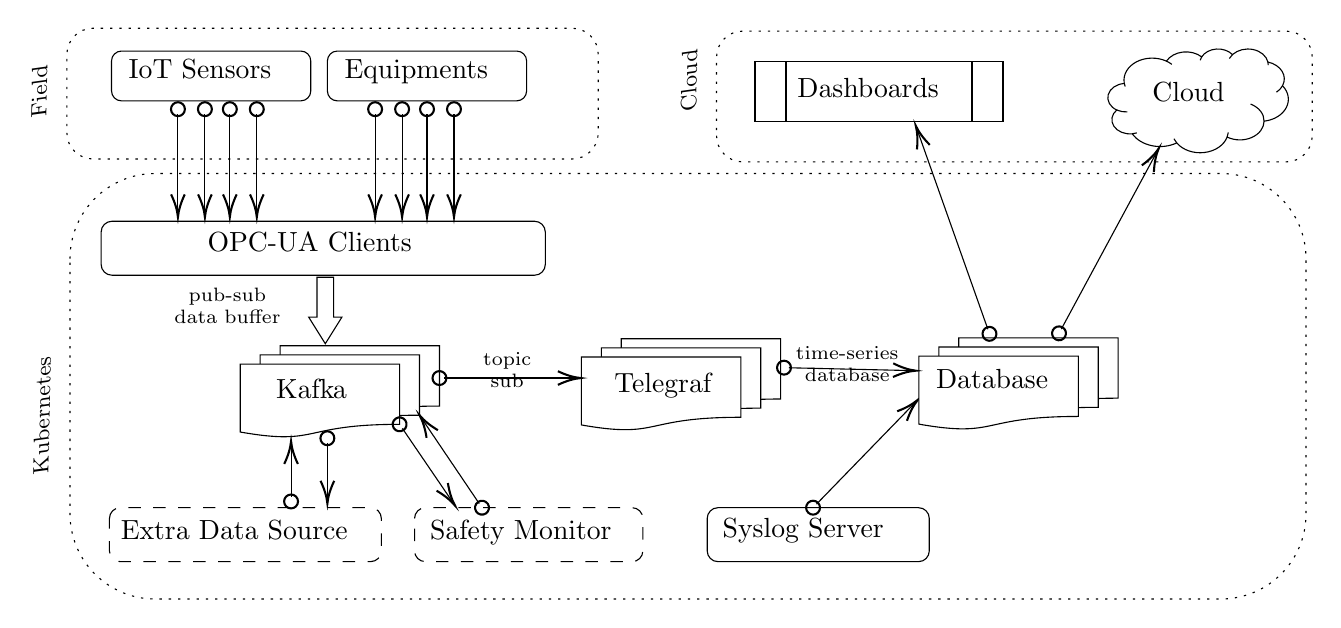
\begin{tikzpicture}[x=0.75pt,y=0.75pt,yscale=-1,xscale=1]
            %uncomment if require: \path (0,433); %set diagram left start at 0, and has height of 433
            
            %Rounded Rect [id:dp8982714762621696] 
            \draw   (55,22.8) .. controls (55,20.15) and (57.15,18) .. (59.8,18) -- (146.2,18) .. controls (148.85,18) and (151,20.15) .. (151,22.8) -- (151,37.2) .. controls (151,39.85) and (148.85,42) .. (146.2,42) -- (59.8,42) .. controls (57.15,42) and (55,39.85) .. (55,37.2) -- cycle ;
            %Rounded Rect [id:dp6816792156669004] 
            \draw   (159,22.8) .. controls (159,20.15) and (161.15,18) .. (163.8,18) -- (250.2,18) .. controls (252.85,18) and (255,20.15) .. (255,22.8) -- (255,37.2) .. controls (255,39.85) and (252.85,42) .. (250.2,42) -- (163.8,42) .. controls (161.15,42) and (159,39.85) .. (159,37.2) -- cycle ;
            %Rounded Rect [id:dp12046665148172042] 
            \draw   (50,105.2) .. controls (50,102.33) and (52.33,100) .. (55.2,100) -- (258.8,100) .. controls (261.67,100) and (264,102.33) .. (264,105.2) -- (264,120.8) .. controls (264,123.67) and (261.67,126) .. (258.8,126) -- (55.2,126) .. controls (52.33,126) and (50,123.67) .. (50,120.8) -- cycle ;
            %Straight Lines [id:da6052410551053385] 
            \draw    (87,48.35) -- (87,96) ;
            \draw [shift={(87,98)}, rotate = 270] [color={rgb, 255:red, 0; green, 0; blue, 0 }  ][line width=0.75]    (10.93,-3.29) .. controls (6.95,-1.4) and (3.31,-0.3) .. (0,0) .. controls (3.31,0.3) and (6.95,1.4) .. (10.93,3.29)   ;
            \draw [shift={(87,46)}, rotate = 90] [color={rgb, 255:red, 0; green, 0; blue, 0 }  ][line width=0.75]      (0, 0) circle [x radius= 3.35, y radius= 3.35]   ;
            %Straight Lines [id:da5587007251053915] 
            \draw    (100,48.35) -- (100,96) ;
            \draw [shift={(100,98)}, rotate = 270] [color={rgb, 255:red, 0; green, 0; blue, 0 }  ][line width=0.75]    (10.93,-3.29) .. controls (6.95,-1.4) and (3.31,-0.3) .. (0,0) .. controls (3.31,0.3) and (6.95,1.4) .. (10.93,3.29)   ;
            \draw [shift={(100,46)}, rotate = 90] [color={rgb, 255:red, 0; green, 0; blue, 0 }  ][line width=0.75]      (0, 0) circle [x radius= 3.35, y radius= 3.35]   ;
            %Straight Lines [id:da8182439450028989] 
            \draw    (112,48.35) -- (112,96) ;
            \draw [shift={(112,98)}, rotate = 270] [color={rgb, 255:red, 0; green, 0; blue, 0 }  ][line width=0.75]    (10.93,-3.29) .. controls (6.95,-1.4) and (3.31,-0.3) .. (0,0) .. controls (3.31,0.3) and (6.95,1.4) .. (10.93,3.29)   ;
            \draw [shift={(112,46)}, rotate = 90] [color={rgb, 255:red, 0; green, 0; blue, 0 }  ][line width=0.75]      (0, 0) circle [x radius= 3.35, y radius= 3.35]   ;
            %Straight Lines [id:da11015490161628927] 
            \draw    (125,48.35) -- (125,96) ;
            \draw [shift={(125,98)}, rotate = 270] [color={rgb, 255:red, 0; green, 0; blue, 0 }  ][line width=0.75]    (10.93,-3.29) .. controls (6.95,-1.4) and (3.31,-0.3) .. (0,0) .. controls (3.31,0.3) and (6.95,1.4) .. (10.93,3.29)   ;
            \draw [shift={(125,46)}, rotate = 90] [color={rgb, 255:red, 0; green, 0; blue, 0 }  ][line width=0.75]      (0, 0) circle [x radius= 3.35, y radius= 3.35]   ;
            %Straight Lines [id:da35591914082952225] 
            \draw    (182,48.35) -- (182,96) ;
            \draw [shift={(182,98)}, rotate = 270] [color={rgb, 255:red, 0; green, 0; blue, 0 }  ][line width=0.75]    (10.93,-3.29) .. controls (6.95,-1.4) and (3.31,-0.3) .. (0,0) .. controls (3.31,0.3) and (6.95,1.4) .. (10.93,3.29)   ;
            \draw [shift={(182,46)}, rotate = 90] [color={rgb, 255:red, 0; green, 0; blue, 0 }  ][line width=0.75]      (0, 0) circle [x radius= 3.35, y radius= 3.35]   ;
            %Straight Lines [id:da7031441556421112] 
            \draw    (195,48.35) -- (195,96) ;
            \draw [shift={(195,98)}, rotate = 270] [color={rgb, 255:red, 0; green, 0; blue, 0 }  ][line width=0.75]    (10.93,-3.29) .. controls (6.95,-1.4) and (3.31,-0.3) .. (0,0) .. controls (3.31,0.3) and (6.95,1.4) .. (10.93,3.29)   ;
            \draw [shift={(195,46)}, rotate = 90] [color={rgb, 255:red, 0; green, 0; blue, 0 }  ][line width=0.75]      (0, 0) circle [x radius= 3.35, y radius= 3.35]   ;
            %Straight Lines [id:da43999440496393993] 
            \draw    (207,48.35) -- (207,96) ;
            \draw [shift={(207,98)}, rotate = 270] [color={rgb, 255:red, 0; green, 0; blue, 0 }  ][line width=0.75]    (10.93,-3.29) .. controls (6.95,-1.4) and (3.31,-0.3) .. (0,0) .. controls (3.31,0.3) and (6.95,1.4) .. (10.93,3.29)   ;
            \draw [shift={(207,46)}, rotate = 90] [color={rgb, 255:red, 0; green, 0; blue, 0 }  ][line width=0.75]      (0, 0) circle [x radius= 3.35, y radius= 3.35]   ;
            %Straight Lines [id:da21849243340929336] 
            \draw    (220,48.35) -- (220,96) ;
            \draw [shift={(220,98)}, rotate = 270] [color={rgb, 255:red, 0; green, 0; blue, 0 }  ][line width=0.75]    (10.93,-3.29) .. controls (6.95,-1.4) and (3.31,-0.3) .. (0,0) .. controls (3.31,0.3) and (6.95,1.4) .. (10.93,3.29)   ;
            \draw [shift={(220,46)}, rotate = 90] [color={rgb, 255:red, 0; green, 0; blue, 0 }  ][line width=0.75]      (0, 0) circle [x radius= 3.35, y radius= 3.35]   ;
            %Down Arrow [id:dp9015495980245107] 
            \draw   (150,146.2) -- (154,146.2) -- (154,127) -- (162,127) -- (162,146.2) -- (166,146.2) -- (158,159) -- cycle ;
            %Rounded Rect [id:dp828856602045485] 
            \draw  [dash pattern={on 4.5pt off 4.5pt}] (201,243.2) .. controls (201,240.33) and (203.33,238) .. (206.2,238) -- (305.8,238) .. controls (308.67,238) and (311,240.33) .. (311,243.2) -- (311,258.8) .. controls (311,261.67) and (308.67,264) .. (305.8,264) -- (206.2,264) .. controls (203.33,264) and (201,261.67) .. (201,258.8) -- cycle ;
            %Straight Lines [id:da9330333745011611] 
            \draw    (159,206.89) -- (159,234) ;
            \draw [shift={(159,236)}, rotate = 270] [color={rgb, 255:red, 0; green, 0; blue, 0 }  ][line width=0.75]    (10.93,-3.29) .. controls (6.95,-1.4) and (3.31,-0.3) .. (0,0) .. controls (3.31,0.3) and (6.95,1.4) .. (10.93,3.29)   ;
            \draw [shift={(159,204.54)}, rotate = 90] [color={rgb, 255:red, 0; green, 0; blue, 0 }  ][line width=0.75]      (0, 0) circle [x radius= 3.35, y radius= 3.35]   ;
            %Rounded Rect [id:dp8994280955151244] 
            \draw   (342,243.2) .. controls (342,240.33) and (344.33,238) .. (347.2,238) -- (443.8,238) .. controls (446.67,238) and (449,240.33) .. (449,243.2) -- (449,258.8) .. controls (449,261.67) and (446.67,264) .. (443.8,264) -- (347.2,264) .. controls (344.33,264) and (342,261.67) .. (342,258.8) -- cycle ;
            %Straight Lines [id:da21801811542650174] 
            \draw    (394.64,236.31) -- (442.11,187.43) ;
            \draw [shift={(443.5,186)}, rotate = 494.16] [color={rgb, 255:red, 0; green, 0; blue, 0 }  ][line width=0.75]    (10.93,-3.29) .. controls (6.95,-1.4) and (3.31,-0.3) .. (0,0) .. controls (3.31,0.3) and (6.95,1.4) .. (10.93,3.29)   ;
            \draw [shift={(393,238)}, rotate = 314.16] [color={rgb, 255:red, 0; green, 0; blue, 0 }  ][line width=0.75]      (0, 0) circle [x radius= 3.35, y radius= 3.35]   ;
            %Shape: Cloud [id:dp1377035889484869] 
            \draw   (542.92,33.46) .. controls (542.22,29.43) and (544.52,25.44) .. (548.84,23.18) .. controls (553.17,20.93) and (558.76,20.8) .. (563.24,22.86) .. controls (564.83,20.51) and (567.74,18.89) .. (571.08,18.49) .. controls (574.43,18.09) and (577.82,18.95) .. (580.24,20.81) .. controls (581.59,18.68) and (584.25,17.25) .. (587.27,17.03) .. controls (590.28,16.81) and (593.24,17.82) .. (595.07,19.71) .. controls (597.52,17.46) and (601.41,16.51) .. (605.06,17.27) .. controls (608.71,18.04) and (611.47,20.38) .. (612.14,23.29) .. controls (615.14,23.93) and (617.63,25.56) .. (618.98,27.75) .. controls (620.33,29.94) and (620.4,32.49) .. (619.18,34.72) .. controls (622.13,37.73) and (622.82,41.74) .. (620.99,45.25) .. controls (619.17,48.76) and (615.1,51.24) .. (610.3,51.78) .. controls (610.27,55.07) and (607.96,58.1) .. (604.27,59.68) .. controls (600.58,61.27) and (596.08,61.17) .. (592.51,59.43) .. controls (590.98,63.37) and (586.7,66.28) .. (581.51,66.88) .. controls (576.31,67.49) and (571.14,65.69) .. (568.22,62.26) .. controls (564.64,63.95) and (560.35,64.44) .. (556.31,63.61) .. controls (552.27,62.79) and (548.82,60.72) .. (546.75,57.87) .. controls (543.09,58.21) and (539.56,56.73) .. (537.9,54.16) .. controls (536.24,51.59) and (536.81,48.49) .. (539.32,46.4) .. controls (536.06,44.89) and (534.4,41.91) .. (535.2,39) .. controls (536,36.1) and (539.08,33.92) .. (542.84,33.62) ; \draw   (539.32,46.39) .. controls (540.86,47.1) and (542.64,47.43) .. (544.42,47.32)(546.75,57.87) .. controls (547.51,57.8) and (548.26,57.66) .. (548.98,57.43)(568.22,62.26) .. controls (567.68,61.63) and (567.23,60.96) .. (566.88,60.25)(592.51,59.43) .. controls (592.78,58.71) and (592.96,57.97) .. (593.04,57.22)(610.3,51.78) .. controls (610.34,48.27) and (607.79,45.06) .. (603.76,43.52)(619.18,34.72) .. controls (618.53,35.92) and (617.53,36.98) .. (616.27,37.82)(612.14,23.29) .. controls (612.25,23.77) and (612.3,24.26) .. (612.29,24.75)(595.07,19.71) .. controls (594.46,20.27) and (593.96,20.9) .. (593.58,21.57)(580.24,20.81) .. controls (579.91,21.32) and (579.67,21.86) .. (579.52,22.42)(563.24,22.86) .. controls (564.19,23.29) and (565.07,23.81) .. (565.85,24.42)(542.92,33.46) .. controls (543.01,34.02) and (543.17,34.57) .. (543.37,35.1) ;
            %Flowchart: Multidocument [id:dp33619279164384785] 
            \draw  [fill={rgb, 255:red, 255; green, 255; blue, 255 }  ,fill opacity=1 ] (136.2,160) -- (213,160) -- (213,189.04) .. controls (165,189.04) and (174.6,199.51) .. (136.2,192.74) -- cycle ; \draw  [fill={rgb, 255:red, 255; green, 255; blue, 255 }  ,fill opacity=1 ] (126.6,164.4) -- (203.4,164.4) -- (203.4,193.44) .. controls (155.4,193.44) and (165,203.91) .. (126.6,197.14) -- cycle ; \draw  [fill={rgb, 255:red, 255; green, 255; blue, 255 }  ,fill opacity=1 ] (117,168.8) -- (193.8,168.8) -- (193.8,197.84) .. controls (145.8,197.84) and (155.4,208.31) .. (117,201.54) -- cycle ;
            %Flowchart: Multidocument [id:dp5205209835800733] 
            \draw  [fill={rgb, 255:red, 255; green, 255; blue, 255 }  ,fill opacity=1 ] (300.6,156.6) -- (377.4,156.6) -- (377.4,185.64) .. controls (329.4,185.64) and (339,196.11) .. (300.6,189.34) -- cycle ; \draw  [fill={rgb, 255:red, 255; green, 255; blue, 255 }  ,fill opacity=1 ] (291,161) -- (367.8,161) -- (367.8,190.04) .. controls (319.8,190.04) and (329.4,200.51) .. (291,193.74) -- cycle ; \draw  [fill={rgb, 255:red, 255; green, 255; blue, 255 }  ,fill opacity=1 ] (281.4,165.4) -- (358.2,165.4) -- (358.2,194.44) .. controls (310.2,194.44) and (319.8,204.91) .. (281.4,198.14) -- cycle ;
            %Flowchart: Multidocument [id:dp8912749746098887] 
            \draw  [fill={rgb, 255:red, 255; green, 255; blue, 255 }  ,fill opacity=1 ] (463.2,156.2) -- (540,156.2) -- (540,185.24) .. controls (492,185.24) and (501.6,195.71) .. (463.2,188.94) -- cycle ; \draw  [fill={rgb, 255:red, 255; green, 255; blue, 255 }  ,fill opacity=1 ] (453.6,160.6) -- (530.4,160.6) -- (530.4,189.64) .. controls (482.4,189.64) and (492,200.11) .. (453.6,193.34) -- cycle ; \draw  [fill={rgb, 255:red, 255; green, 255; blue, 255 }  ,fill opacity=1 ] (444,165) -- (520.8,165) -- (520.8,194.04) .. controls (472.8,194.04) and (482.4,204.51) .. (444,197.74) -- cycle ;
            %Straight Lines [id:da2725348840465214] 
            \draw    (477.22,152.02) -- (443.17,55.89) ;
            \draw [shift={(442.5,54)}, rotate = 430.5] [color={rgb, 255:red, 0; green, 0; blue, 0 }  ][line width=0.75]    (10.93,-3.29) .. controls (6.95,-1.4) and (3.31,-0.3) .. (0,0) .. controls (3.31,0.3) and (6.95,1.4) .. (10.93,3.29)   ;
            \draw [shift={(478,154.24)}, rotate = 250.5] [color={rgb, 255:red, 0; green, 0; blue, 0 }  ][line width=0.75]      (0, 0) circle [x radius= 3.35, y radius= 3.35]   ;
            %Straight Lines [id:da6479961353344621] 
            \draw    (215.35,175.54) -- (279,175.54) ;
            \draw [shift={(281,175.54)}, rotate = 180] [color={rgb, 255:red, 0; green, 0; blue, 0 }  ][line width=0.75]    (10.93,-3.29) .. controls (6.95,-1.4) and (3.31,-0.3) .. (0,0) .. controls (3.31,0.3) and (6.95,1.4) .. (10.93,3.29)   ;
            \draw [shift={(213,175.54)}, rotate = 0] [color={rgb, 255:red, 0; green, 0; blue, 0 }  ][line width=0.75]      (0, 0) circle [x radius= 3.35, y radius= 3.35]   ;
            %Rounded Rect [id:dp5935934620458618] 
            \draw  [dash pattern={on 4.5pt off 4.5pt}] (54,243.2) .. controls (54,240.33) and (56.33,238) .. (59.2,238) -- (179.8,238) .. controls (182.67,238) and (185,240.33) .. (185,243.2) -- (185,258.8) .. controls (185,261.67) and (182.67,264) .. (179.8,264) -- (59.2,264) .. controls (56.33,264) and (54,261.67) .. (54,258.8) -- cycle ;
            %Straight Lines [id:da8930686223033689] 
            \draw    (141.5,232.65) -- (141.5,208) ;
            \draw [shift={(141.5,206)}, rotate = 450] [color={rgb, 255:red, 0; green, 0; blue, 0 }  ][line width=0.75]    (10.93,-3.29) .. controls (6.95,-1.4) and (3.31,-0.3) .. (0,0) .. controls (3.31,0.3) and (6.95,1.4) .. (10.93,3.29)   ;
            \draw [shift={(141.5,235)}, rotate = 270] [color={rgb, 255:red, 0; green, 0; blue, 0 }  ][line width=0.75]      (0, 0) circle [x radius= 3.35, y radius= 3.35]   ;
            %Straight Lines [id:da03433104300151424] 
            \draw    (195.12,199.78) -- (219.37,235.35) ;
            \draw [shift={(220.5,237)}, rotate = 235.71] [color={rgb, 255:red, 0; green, 0; blue, 0 }  ][line width=0.75]    (10.93,-3.29) .. controls (6.95,-1.4) and (3.31,-0.3) .. (0,0) .. controls (3.31,0.3) and (6.95,1.4) .. (10.93,3.29)   ;
            \draw [shift={(193.8,197.84)}, rotate = 55.71] [color={rgb, 255:red, 0; green, 0; blue, 0 }  ][line width=0.75]      (0, 0) circle [x radius= 3.35, y radius= 3.35]   ;
            %Straight Lines [id:da4851968248935681] 
            \draw    (232.18,236.05) -- (204.52,195.1) ;
            \draw [shift={(203.4,193.44)}, rotate = 415.96000000000004] [color={rgb, 255:red, 0; green, 0; blue, 0 }  ][line width=0.75]    (10.93,-3.29) .. controls (6.95,-1.4) and (3.31,-0.3) .. (0,0) .. controls (3.31,0.3) and (6.95,1.4) .. (10.93,3.29)   ;
            \draw [shift={(233.5,238)}, rotate = 235.96] [color={rgb, 255:red, 0; green, 0; blue, 0 }  ][line width=0.75]      (0, 0) circle [x radius= 3.35, y radius= 3.35]   ;
            %Straight Lines [id:da0384301657035514] 
            \draw    (381.35,170.59) -- (440.5,171.95) ;
            \draw [shift={(442.5,172)}, rotate = 181.32] [color={rgb, 255:red, 0; green, 0; blue, 0 }  ][line width=0.75]    (10.93,-3.29) .. controls (6.95,-1.4) and (3.31,-0.3) .. (0,0) .. controls (3.31,0.3) and (6.95,1.4) .. (10.93,3.29)   ;
            \draw [shift={(379,170.54)}, rotate = 1.32] [color={rgb, 255:red, 0; green, 0; blue, 0 }  ][line width=0.75]      (0, 0) circle [x radius= 3.35, y radius= 3.35]   ;
            %Flowchart: Prodefined Process [id:dp9461366879112181] 
            \draw   (365,23) -- (484.5,23) -- (484.5,52) -- (365,52) -- cycle ; \draw   (379.94,23) -- (379.94,52) ; \draw   (469.56,23) -- (469.56,52) ;
            %Straight Lines [id:da055997175321346404] 
            \draw    (512.62,151.93) -- (558.55,66.76) ;
            \draw [shift={(559.5,65)}, rotate = 478.34] [color={rgb, 255:red, 0; green, 0; blue, 0 }  ][line width=0.75]    (10.93,-3.29) .. controls (6.95,-1.4) and (3.31,-0.3) .. (0,0) .. controls (3.31,0.3) and (6.95,1.4) .. (10.93,3.29)   ;
            \draw [shift={(511.5,154)}, rotate = 298.34] [color={rgb, 255:red, 0; green, 0; blue, 0 }  ][line width=0.75]      (0, 0) circle [x radius= 3.35, y radius= 3.35]   ;
            %Rounded Rect [id:dp7059673720575631] 
            \draw  [dash pattern={on 0.84pt off 2.51pt}] (35,118) .. controls (35,95.36) and (53.36,77) .. (76,77) -- (589.5,77) .. controls (612.14,77) and (630.5,95.36) .. (630.5,118) -- (630.5,241) .. controls (630.5,263.64) and (612.14,282) .. (589.5,282) -- (76,282) .. controls (53.36,282) and (35,263.64) .. (35,241) -- cycle ;
            %Rounded Rect [id:dp5779436854653599] 
            \draw  [dash pattern={on 0.84pt off 2.51pt}] (33.5,57.4) .. controls (33.5,64.36) and (39.14,70) .. (46.1,70) -- (276.9,70) .. controls (283.86,70) and (289.5,64.36) .. (289.5,57.4) -- (289.5,19.6) .. controls (289.5,12.64) and (283.86,7) .. (276.9,7) -- (46.1,7) .. controls (39.14,7) and (33.5,12.64) .. (33.5,19.6) -- cycle ;
            %Rounded Rect [id:dp48214793802537337] 
            \draw  [dash pattern={on 0.84pt off 2.51pt}] (346.5,58.8) .. controls (346.5,65.76) and (352.14,71.4) .. (359.1,71.4) -- (620.9,71.4) .. controls (627.86,71.4) and (633.5,65.76) .. (633.5,58.8) -- (633.5,21) .. controls (633.5,14.04) and (627.86,8.4) .. (620.9,8.4) -- (359.1,8.4) .. controls (352.14,8.4) and (346.5,14.04) .. (346.5,21) -- cycle ;
            
            % Text Node
            \draw (62,21) node [anchor=north west][inner sep=0.75pt]   [align=left] {IoT Sensors};
            % Text Node
            \draw (166,21) node [anchor=north west][inner sep=0.75pt]   [align=left] {Equipments};
            % Text Node
            \draw (100,104) node [anchor=north west][inner sep=0.75pt]   [align=left] {OPC-UA Clients};
            % Text Node
            \draw (84,131) node [anchor=north west][inner sep=0.75pt]  [font=\scriptsize] [align=left] {\begin{minipage}[lt]{38.35625pt}\setlength\topsep{0pt}
                    \begin{center}
                        pub-sub\\data buffer
                    \end{center}
                    
            \end{minipage}};
            % Text Node
            \draw (207.2,243) node [anchor=north west][inner sep=0.75pt]   [align=left] {Safety Monitor};
            % Text Node
            \draw (232,162) node [anchor=north west][inner sep=0.75pt]  [font=\scriptsize] [align=left] {\begin{minipage}[lt]{18.53pt}\setlength\topsep{0pt}
                    \begin{center}
                        topic\\sub
                    \end{center}
                    
            \end{minipage}};
            % Text Node
            \draw (382,159) node [anchor=north west][inner sep=0.75pt]  [font=\scriptsize] [align=left] {\begin{minipage}[lt]{39.301875pt}\setlength\topsep{0pt}
                    \begin{center}
                        time-series\\database
                    \end{center}
                    
            \end{minipage}};
            % Text Node
            \draw (348.2,242) node [anchor=north west][inner sep=0.75pt]   [align=left] {Syslog Server};
            % Text Node
            \draw (555.2,32) node [anchor=north west][inner sep=0.75pt]   [align=left] {Cloud};
            % Text Node
            \draw (133,175) node [anchor=north west][inner sep=0.75pt]   [align=left] {Kafka};
            % Text Node
            \draw (296,172) node [anchor=north west][inner sep=0.75pt]   [align=left] {Telegraf};
            % Text Node
            \draw (384.2,30) node [anchor=north west][inner sep=0.75pt]   [align=left] {Dashboards};
            % Text Node
            \draw (451,170) node [anchor=north west][inner sep=0.75pt]   [align=left] {Database};
            % Text Node
            \draw (58.2,243) node [anchor=north west][inner sep=0.75pt]   [align=left] {Extra Data Source};
            % Text Node
            \draw (15.87,225.25) node [anchor=north west][inner sep=0.75pt]  [font=\footnotesize,rotate=-271.22,xslant=-0.16] [align=left] {\begin{minipage}[lt]{44.465625pt}\setlength\topsep{0pt}
                    \begin{center}
                        Kubernetes
                    \end{center}
                    
            \end{minipage}};
            % Text Node
            \draw (14.87,53.25) node [anchor=north west][inner sep=0.75pt]  [font=\footnotesize,rotate=-271.22,xslant=-0.16] [align=left] {\begin{minipage}[lt]{20.410625000000003pt}\setlength\topsep{0pt}
                    \begin{center}
                        Field
                    \end{center}
                    
            \end{minipage}};
            % Text Node
            \draw (327.87,50.25) node [anchor=north west][inner sep=0.75pt]  [font=\footnotesize,rotate=-271.22,xslant=-0.16] [align=left] {\begin{minipage}[lt]{24.044375000000002pt}\setlength\topsep{0pt}
                    \begin{center}
                        Cloud
                    \end{center}
                    
            \end{minipage}};
            
            
        \end{tikzpicture}
           
        \caption{A high-level view of the state-of-the-art ICE lab data collection architecture}
         \label{DataCollectionArchitecture}
    \end{figure*}
    
    \section{ICE LAB Architecture}
Currently, at the state of the art, the ICE lab uses a data collection architecture based on Kubernetes and OPC-UA with the goal of performing monitoring operations, logging, and analyzing the plant status.
       
       ICE lab has three separate servers on which to keep the architecture active. Specifically, they use k3s, a distribution of Kubernetes created ad hoc for IoT and Edge Computing, and is it running on the following hardware configuration:
       
       \begin{itemize}
           \item Intel Core i5-3470
           \item 3x 8GB DDR3 1600MHz
           \item Ubuntu Server
           \end{itemize}
           And two edge boards:
                      \begin{itemize}
           \item Atom E3940 1Ghz 4core
           \item 2GB RAM
       \end{itemize}
   
   Meanwhile the figure ~\ref{DataCollectionArchitecture} shows an high-level view of the ICE lab data collection architecture.
   
   Is possible to see three different areas: the \textit{field} area, where data is generated by the various clients (such as the Kuka robot, the production line, and/or the 3d printers) which use the OPC-UA protocol to communicate with the architecture; the \textit{kubernetes} area, where all the core architecture and data collection services reside; and the \textit{cloud} area, where the dashboards and analysis tools from \textit{PaaS} are located (e.g. Siemens cloud).

\section{ICE LAB Data flow}
Referring again to the figure ~\ref{DataCollectionArchitecture}, it is quite clear to understand what is the data flow:
OPC-UA clients generate data and communicate it to the respective server, i.e. a pod running an OPC-UA service initialized within the k3s architecture.
This data, subsequently, passes within the heart of this architecture: Kafka.
Apache Kafka ~\cite{kafkaOfficial} is an event stream platform, which combines three key capabilities so you can implement your use cases for event streaming end-to-end with a single battle-tested solution, e.g.:

\begin{itemize}
    \item To publish (write) and subscribe to (read) streams of events, including continuous import/export of your data from other systems;
    \item To store streams of events durably and reliably for as long as you want;
    \item To process streams of events as they occur or retrospectively.
\end{itemize}
So, Apache Kafka, thanks to the public-subscriber protocol, become the main broker of the architecture: all clients that will send data to Kafka will be publishers, as in this case, the OPC-UA server clients, while, clients like the safety monitor, or Telegraf, which will consume data, will be consumers.


In order to take the data from Kafka and put it on the InfluxDB database, a tool was needed to act as a consumer and redirect the data to InfluxDB. For this purpose, Telegraf is used.

Telegraf is a server agent written in Go that relies on plugins to collect and send metrics from a variety of input systems to InfluxDB. It allows you to collect data written in different formats and is very versatile, as to add a new input system, you simply need to download the relevant plugin and edit the configuration file.


In our case, Telegraf is in charge of consuming topics from an Apache Kafka server using the related plugin and uploading the data to a dedicated InfluxDB bucket. 
\\

The data flow then ends up in InfluxDB, a time-series database that can boast of being able to handle up to 1 million writes per second ~\cite{influx}. Other applications (such as ICETOM ~\cite{icetom}) will then upload the InfluxDB data to a cloud (e.g. Siemens Cloud) for data analysis or dashboards.

All nodes, within the area Kubernetes visible in figure ~\ref{DataCollectionArchitecture}, have the ability to take advantage of the replication techniques, which allow you to quickly scale horizontally the same pod. This leads to better performance and self-balancing thanks to k3s when a node is too overloaded.

\begin{figure*}[ht]
    \centering
    

\tikzset{every picture/.style={line width=0.75pt}} %set default line width to 0.75pt        

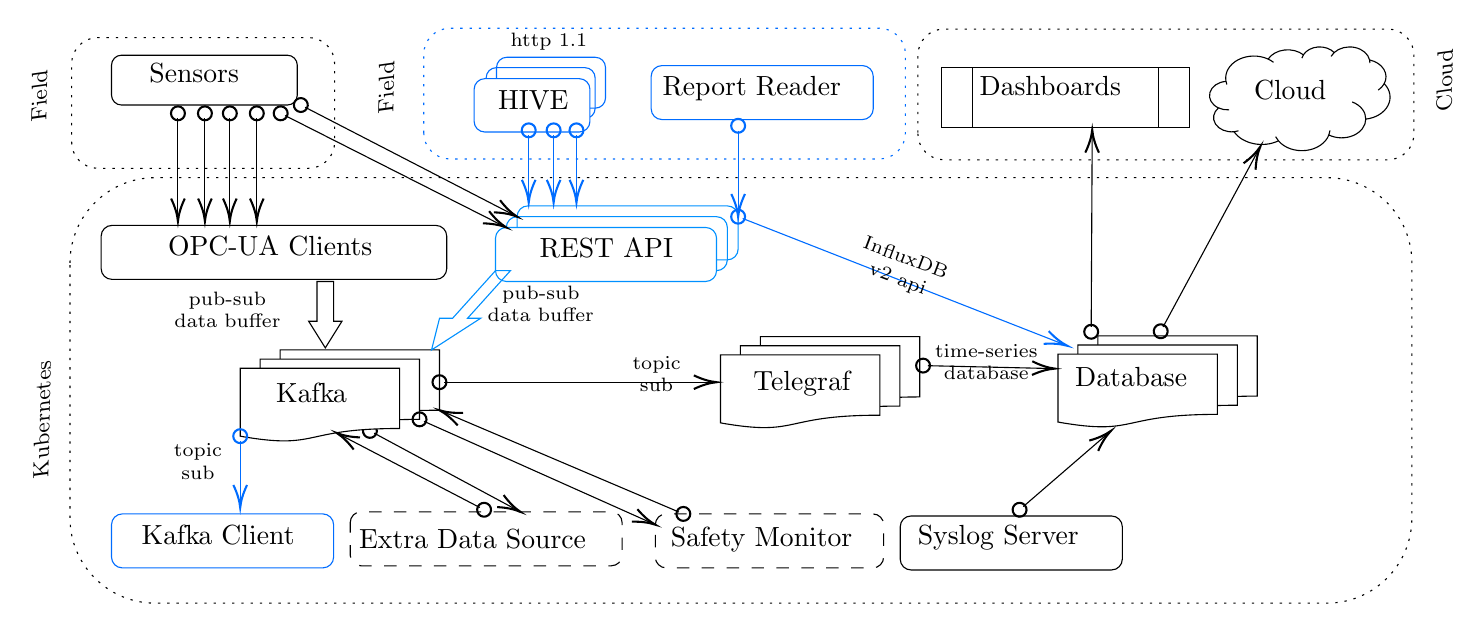
\begin{tikzpicture}[x=0.75pt,y=0.75pt,yscale=-1,xscale=1]
%uncomment if require: \path (0,317); %set diagram left start at 0, and has height of 317

%Rounded Rect [id:dp52590233517953] 
\draw  [color={rgb, 255:red, 0; green, 108; blue, 255 }  ,draw opacity=1 ] (250.5,30.9) .. controls (250.5,28.19) and (252.69,26) .. (255.4,26) -- (298.1,26) .. controls (300.81,26) and (303,28.19) .. (303,30.9) -- (303,45.6) .. controls (303,48.31) and (300.81,50.5) .. (298.1,50.5) -- (255.4,50.5) .. controls (252.69,50.5) and (250.5,48.31) .. (250.5,45.6) -- cycle ;
%Rounded Rect [id:dp9870595909973515] 
\draw  [color={rgb, 255:red, 0; green, 144; blue, 255 }  ,draw opacity=1 ] (260.4,102.8) .. controls (260.4,99.93) and (262.73,97.6) .. (265.6,97.6) -- (361.7,97.6) .. controls (364.57,97.6) and (366.9,99.93) .. (366.9,102.8) -- (366.9,118.4) .. controls (366.9,121.27) and (364.57,123.6) .. (361.7,123.6) -- (265.6,123.6) .. controls (262.73,123.6) and (260.4,121.27) .. (260.4,118.4) -- cycle ;
%Rounded Rect [id:dp7829018277211611] 
\draw  [color={rgb, 255:red, 0; green, 144; blue, 255 }  ,draw opacity=1 ] (255.2,108) .. controls (255.2,105.13) and (257.53,102.8) .. (260.4,102.8) -- (356.5,102.8) .. controls (359.37,102.8) and (361.7,105.13) .. (361.7,108) -- (361.7,123.6) .. controls (361.7,126.47) and (359.37,128.8) .. (356.5,128.8) -- (260.4,128.8) .. controls (257.53,128.8) and (255.2,126.47) .. (255.2,123.6) -- cycle ;
%Rounded Rect [id:dp8982714762621696] 
\draw   (65,29.8) .. controls (65,27.15) and (67.15,25) .. (69.8,25) -- (149.7,25) .. controls (152.35,25) and (154.5,27.15) .. (154.5,29.8) -- (154.5,44.2) .. controls (154.5,46.85) and (152.35,49) .. (149.7,49) -- (69.8,49) .. controls (67.15,49) and (65,46.85) .. (65,44.2) -- cycle ;
%Rounded Rect [id:dp12046665148172042] 
\draw   (60,112.2) .. controls (60,109.33) and (62.33,107) .. (65.2,107) -- (221.3,107) .. controls (224.17,107) and (226.5,109.33) .. (226.5,112.2) -- (226.5,127.8) .. controls (226.5,130.67) and (224.17,133) .. (221.3,133) -- (65.2,133) .. controls (62.33,133) and (60,130.67) .. (60,127.8) -- cycle ;
%Straight Lines [id:da6052410551053385] 
\draw    (97,55.35) -- (97,103) ;
\draw [shift={(97,105)}, rotate = 270] [color={rgb, 255:red, 0; green, 0; blue, 0 }  ][line width=0.75]    (10.93,-3.29) .. controls (6.95,-1.4) and (3.31,-0.3) .. (0,0) .. controls (3.31,0.3) and (6.95,1.4) .. (10.93,3.29)   ;
\draw [shift={(97,53)}, rotate = 90] [color={rgb, 255:red, 0; green, 0; blue, 0 }  ][line width=0.75]      (0, 0) circle [x radius= 3.35, y radius= 3.35]   ;
%Straight Lines [id:da5587007251053915] 
\draw    (110,55.35) -- (110,103) ;
\draw [shift={(110,105)}, rotate = 270] [color={rgb, 255:red, 0; green, 0; blue, 0 }  ][line width=0.75]    (10.93,-3.29) .. controls (6.95,-1.4) and (3.31,-0.3) .. (0,0) .. controls (3.31,0.3) and (6.95,1.4) .. (10.93,3.29)   ;
\draw [shift={(110,53)}, rotate = 90] [color={rgb, 255:red, 0; green, 0; blue, 0 }  ][line width=0.75]      (0, 0) circle [x radius= 3.35, y radius= 3.35]   ;
%Straight Lines [id:da8182439450028989] 
\draw    (122,55.35) -- (122,103) ;
\draw [shift={(122,105)}, rotate = 270] [color={rgb, 255:red, 0; green, 0; blue, 0 }  ][line width=0.75]    (10.93,-3.29) .. controls (6.95,-1.4) and (3.31,-0.3) .. (0,0) .. controls (3.31,0.3) and (6.95,1.4) .. (10.93,3.29)   ;
\draw [shift={(122,53)}, rotate = 90] [color={rgb, 255:red, 0; green, 0; blue, 0 }  ][line width=0.75]      (0, 0) circle [x radius= 3.35, y radius= 3.35]   ;
%Straight Lines [id:da11015490161628927] 
\draw    (135,55.35) -- (135,103) ;
\draw [shift={(135,105)}, rotate = 270] [color={rgb, 255:red, 0; green, 0; blue, 0 }  ][line width=0.75]    (10.93,-3.29) .. controls (6.95,-1.4) and (3.31,-0.3) .. (0,0) .. controls (3.31,0.3) and (6.95,1.4) .. (10.93,3.29)   ;
\draw [shift={(135,53)}, rotate = 90] [color={rgb, 255:red, 0; green, 0; blue, 0 }  ][line width=0.75]      (0, 0) circle [x radius= 3.35, y radius= 3.35]   ;
%Down Arrow [id:dp9015495980245107] 
\draw   (160,153.2) -- (164,153.2) -- (164,134) -- (172,134) -- (172,153.2) -- (176,153.2) -- (168,166) -- cycle ;
%Rounded Rect [id:dp828856602045485] 
\draw  [dash pattern={on 4.5pt off 4.5pt}] (327,251.2) .. controls (327,248.33) and (329.33,246) .. (332.2,246) -- (431.8,246) .. controls (434.67,246) and (437,248.33) .. (437,251.2) -- (437,266.8) .. controls (437,269.67) and (434.67,272) .. (431.8,272) -- (332.2,272) .. controls (329.33,272) and (327,269.67) .. (327,266.8) -- cycle ;
%Straight Lines [id:da9330333745011611] 
\draw    (191.57,207.11) -- (260.24,244.05) ;
\draw [shift={(262,245)}, rotate = 208.28] [color={rgb, 255:red, 0; green, 0; blue, 0 }  ][line width=0.75]    (10.93,-3.29) .. controls (6.95,-1.4) and (3.31,-0.3) .. (0,0) .. controls (3.31,0.3) and (6.95,1.4) .. (10.93,3.29)   ;
\draw [shift={(189.5,206)}, rotate = 28.28] [color={rgb, 255:red, 0; green, 0; blue, 0 }  ][line width=0.75]      (0, 0) circle [x radius= 3.35, y radius= 3.35]   ;
%Rounded Rect [id:dp8994280955151244] 
\draw   (445,252.2) .. controls (445,249.33) and (447.33,247) .. (450.2,247) -- (546.8,247) .. controls (549.67,247) and (552,249.33) .. (552,252.2) -- (552,267.8) .. controls (552,270.67) and (549.67,273) .. (546.8,273) -- (450.2,273) .. controls (447.33,273) and (445,270.67) .. (445,267.8) -- cycle ;
%Straight Lines [id:da21801811542650174] 
\draw    (504.28,242.46) -- (544.99,207.31) ;
\draw [shift={(546.5,206)}, rotate = 499.18] [color={rgb, 255:red, 0; green, 0; blue, 0 }  ][line width=0.75]    (10.93,-3.29) .. controls (6.95,-1.4) and (3.31,-0.3) .. (0,0) .. controls (3.31,0.3) and (6.95,1.4) .. (10.93,3.29)   ;
\draw [shift={(502.5,244)}, rotate = 319.18] [color={rgb, 255:red, 0; green, 0; blue, 0 }  ][line width=0.75]      (0, 0) circle [x radius= 3.35, y radius= 3.35]   ;
%Shape: Cloud [id:dp1377035889484869] 
\draw   (601.92,37.46) .. controls (601.22,33.43) and (603.52,29.44) .. (607.84,27.18) .. controls (612.17,24.93) and (617.76,24.8) .. (622.24,26.86) .. controls (623.83,24.51) and (626.74,22.89) .. (630.08,22.49) .. controls (633.43,22.09) and (636.82,22.95) .. (639.24,24.81) .. controls (640.59,22.68) and (643.25,21.25) .. (646.27,21.03) .. controls (649.28,20.81) and (652.24,21.82) .. (654.07,23.71) .. controls (656.52,21.46) and (660.41,20.51) .. (664.06,21.27) .. controls (667.71,22.04) and (670.47,24.38) .. (671.14,27.29) .. controls (674.14,27.93) and (676.63,29.56) .. (677.98,31.75) .. controls (679.33,33.94) and (679.4,36.49) .. (678.18,38.72) .. controls (681.13,41.73) and (681.82,45.74) .. (679.99,49.25) .. controls (678.17,52.76) and (674.1,55.24) .. (669.3,55.78) .. controls (669.27,59.07) and (666.96,62.1) .. (663.27,63.68) .. controls (659.58,65.27) and (655.08,65.17) .. (651.51,63.43) .. controls (649.98,67.37) and (645.7,70.28) .. (640.51,70.88) .. controls (635.31,71.49) and (630.14,69.69) .. (627.22,66.26) .. controls (623.64,67.95) and (619.35,68.44) .. (615.31,67.61) .. controls (611.27,66.79) and (607.82,64.72) .. (605.75,61.87) .. controls (602.09,62.21) and (598.56,60.73) .. (596.9,58.16) .. controls (595.24,55.59) and (595.81,52.49) .. (598.32,50.4) .. controls (595.06,48.89) and (593.4,45.91) .. (594.2,43) .. controls (595,40.1) and (598.08,37.92) .. (601.84,37.62) ; \draw   (598.32,50.39) .. controls (599.86,51.1) and (601.64,51.43) .. (603.42,51.32)(605.75,61.87) .. controls (606.51,61.8) and (607.26,61.66) .. (607.98,61.43)(627.22,66.26) .. controls (626.68,65.63) and (626.23,64.96) .. (625.88,64.25)(651.51,63.43) .. controls (651.78,62.71) and (651.96,61.97) .. (652.04,61.22)(669.3,55.78) .. controls (669.34,52.27) and (666.79,49.06) .. (662.76,47.52)(678.18,38.72) .. controls (677.53,39.92) and (676.53,40.98) .. (675.27,41.82)(671.14,27.29) .. controls (671.25,27.77) and (671.3,28.26) .. (671.29,28.75)(654.07,23.71) .. controls (653.46,24.27) and (652.96,24.9) .. (652.58,25.57)(639.24,24.81) .. controls (638.91,25.32) and (638.67,25.86) .. (638.52,26.42)(622.24,26.86) .. controls (623.19,27.29) and (624.07,27.81) .. (624.85,28.42)(601.92,37.46) .. controls (602.01,38.02) and (602.17,38.57) .. (602.37,39.1) ;
%Flowchart: Multidocument [id:dp33619279164384785] 
\draw  [fill={rgb, 255:red, 255; green, 255; blue, 255 }  ,fill opacity=1 ] (146.2,167) -- (223,167) -- (223,196.04) .. controls (175,196.04) and (184.6,206.51) .. (146.2,199.74) -- cycle ; \draw  [fill={rgb, 255:red, 255; green, 255; blue, 255 }  ,fill opacity=1 ] (136.6,171.4) -- (213.4,171.4) -- (213.4,200.44) .. controls (165.4,200.44) and (175,210.91) .. (136.6,204.14) -- cycle ; \draw  [fill={rgb, 255:red, 255; green, 255; blue, 255 }  ,fill opacity=1 ] (127,175.8) -- (203.8,175.8) -- (203.8,204.84) .. controls (155.8,204.84) and (165.4,215.31) .. (127,208.54) -- cycle ;
%Flowchart: Multidocument [id:dp5205209835800733] 
\draw  [fill={rgb, 255:red, 255; green, 255; blue, 255 }  ,fill opacity=1 ] (377.6,160.6) -- (454.4,160.6) -- (454.4,189.64) .. controls (406.4,189.64) and (416,200.11) .. (377.6,193.34) -- cycle ; \draw  [fill={rgb, 255:red, 255; green, 255; blue, 255 }  ,fill opacity=1 ] (368,165) -- (444.8,165) -- (444.8,194.04) .. controls (396.8,194.04) and (406.4,204.51) .. (368,197.74) -- cycle ; \draw  [fill={rgb, 255:red, 255; green, 255; blue, 255 }  ,fill opacity=1 ] (358.4,169.4) -- (435.2,169.4) -- (435.2,198.44) .. controls (387.2,198.44) and (396.8,208.91) .. (358.4,202.14) -- cycle ;
%Flowchart: Multidocument [id:dp8912749746098887] 
\draw  [fill={rgb, 255:red, 255; green, 255; blue, 255 }  ,fill opacity=1 ] (540.2,160.2) -- (617,160.2) -- (617,189.24) .. controls (569,189.24) and (578.6,199.71) .. (540.2,192.94) -- cycle ; \draw  [fill={rgb, 255:red, 255; green, 255; blue, 255 }  ,fill opacity=1 ] (530.6,164.6) -- (607.4,164.6) -- (607.4,193.64) .. controls (559.4,193.64) and (569,204.11) .. (530.6,197.34) -- cycle ; \draw  [fill={rgb, 255:red, 255; green, 255; blue, 255 }  ,fill opacity=1 ] (521,169) -- (597.8,169) -- (597.8,198.04) .. controls (549.8,198.04) and (559.4,208.51) .. (521,201.74) -- cycle ;
%Straight Lines [id:da2725348840465214] 
\draw    (537.01,155.89) -- (537.49,63) ;
\draw [shift={(537.5,61)}, rotate = 450.29] [color={rgb, 255:red, 0; green, 0; blue, 0 }  ][line width=0.75]    (10.93,-3.29) .. controls (6.95,-1.4) and (3.31,-0.3) .. (0,0) .. controls (3.31,0.3) and (6.95,1.4) .. (10.93,3.29)   ;
\draw [shift={(537,158.24)}, rotate = 270.29] [color={rgb, 255:red, 0; green, 0; blue, 0 }  ][line width=0.75]      (0, 0) circle [x radius= 3.35, y radius= 3.35]   ;
%Straight Lines [id:da6479961353344621] 
\draw    (225.35,182.54) -- (354.5,182.54) ;
\draw [shift={(356.5,182.54)}, rotate = 180] [color={rgb, 255:red, 0; green, 0; blue, 0 }  ][line width=0.75]    (10.93,-3.29) .. controls (6.95,-1.4) and (3.31,-0.3) .. (0,0) .. controls (3.31,0.3) and (6.95,1.4) .. (10.93,3.29)   ;
\draw [shift={(223,182.54)}, rotate = 0] [color={rgb, 255:red, 0; green, 0; blue, 0 }  ][line width=0.75]      (0, 0) circle [x radius= 3.35, y radius= 3.35]   ;
%Rounded Rect [id:dp5935934620458618] 
\draw  [dash pattern={on 4.5pt off 4.5pt}] (180,250.2) .. controls (180,247.33) and (182.33,245) .. (185.2,245) -- (305.8,245) .. controls (308.67,245) and (311,247.33) .. (311,250.2) -- (311,265.8) .. controls (311,268.67) and (308.67,271) .. (305.8,271) -- (185.2,271) .. controls (182.33,271) and (180,268.67) .. (180,265.8) -- cycle ;
%Straight Lines [id:da8930686223033689] 
\draw    (242.42,242.91) -- (175.27,207.92) ;
\draw [shift={(173.5,207)}, rotate = 387.53] [color={rgb, 255:red, 0; green, 0; blue, 0 }  ][line width=0.75]    (10.93,-3.29) .. controls (6.95,-1.4) and (3.31,-0.3) .. (0,0) .. controls (3.31,0.3) and (6.95,1.4) .. (10.93,3.29)   ;
\draw [shift={(244.5,244)}, rotate = 207.53] [color={rgb, 255:red, 0; green, 0; blue, 0 }  ][line width=0.75]      (0, 0) circle [x radius= 3.35, y radius= 3.35]   ;
%Straight Lines [id:da03433104300151424] 
\draw    (215.55,201.4) -- (325.17,250.38) ;
\draw [shift={(327,251.2)}, rotate = 204.07999999999998] [color={rgb, 255:red, 0; green, 0; blue, 0 }  ][line width=0.75]    (10.93,-3.29) .. controls (6.95,-1.4) and (3.31,-0.3) .. (0,0) .. controls (3.31,0.3) and (6.95,1.4) .. (10.93,3.29)   ;
\draw [shift={(213.4,200.44)}, rotate = 24.08] [color={rgb, 255:red, 0; green, 0; blue, 0 }  ][line width=0.75]      (0, 0) circle [x radius= 3.35, y radius= 3.35]   ;
%Straight Lines [id:da4851968248935681] 
\draw    (338.34,245.08) -- (224.84,196.82) ;
\draw [shift={(223,196.04)}, rotate = 383.03] [color={rgb, 255:red, 0; green, 0; blue, 0 }  ][line width=0.75]    (10.93,-3.29) .. controls (6.95,-1.4) and (3.31,-0.3) .. (0,0) .. controls (3.31,0.3) and (6.95,1.4) .. (10.93,3.29)   ;
\draw [shift={(340.5,246)}, rotate = 203.03] [color={rgb, 255:red, 0; green, 0; blue, 0 }  ][line width=0.75]      (0, 0) circle [x radius= 3.35, y radius= 3.35]   ;
%Straight Lines [id:da0384301657035514] 
\draw    (458.35,174.59) -- (517.5,175.95) ;
\draw [shift={(519.5,176)}, rotate = 181.32] [color={rgb, 255:red, 0; green, 0; blue, 0 }  ][line width=0.75]    (10.93,-3.29) .. controls (6.95,-1.4) and (3.31,-0.3) .. (0,0) .. controls (3.31,0.3) and (6.95,1.4) .. (10.93,3.29)   ;
\draw [shift={(456,174.54)}, rotate = 1.32] [color={rgb, 255:red, 0; green, 0; blue, 0 }  ][line width=0.75]      (0, 0) circle [x radius= 3.35, y radius= 3.35]   ;
%Flowchart: Prodefined Process [id:dp9461366879112181] 
\draw   (465,31) -- (584.5,31) -- (584.5,60) -- (465,60) -- cycle ; \draw   (479.94,31) -- (479.94,60) ; \draw   (569.56,31) -- (569.56,60) ;
%Straight Lines [id:da055997175321346404] 
\draw    (571.62,155.93) -- (617.55,70.76) ;
\draw [shift={(618.5,69)}, rotate = 478.34] [color={rgb, 255:red, 0; green, 0; blue, 0 }  ][line width=0.75]    (10.93,-3.29) .. controls (6.95,-1.4) and (3.31,-0.3) .. (0,0) .. controls (3.31,0.3) and (6.95,1.4) .. (10.93,3.29)   ;
\draw [shift={(570.5,158)}, rotate = 298.34] [color={rgb, 255:red, 0; green, 0; blue, 0 }  ][line width=0.75]      (0, 0) circle [x radius= 3.35, y radius= 3.35]   ;
%Rounded Rect [id:dp7059673720575631] 
\draw  [dash pattern={on 0.84pt off 2.51pt}] (45,125) .. controls (45,102.36) and (63.36,84) .. (86,84) -- (650.5,84) .. controls (673.14,84) and (691.5,102.36) .. (691.5,125) -- (691.5,248) .. controls (691.5,270.64) and (673.14,289) .. (650.5,289) -- (86,289) .. controls (63.36,289) and (45,270.64) .. (45,248) -- cycle ;
%Rounded Rect [id:dp5779436854653599] 
\draw  [dash pattern={on 0.84pt off 2.51pt}] (45.8,66.9) .. controls (45.8,73.86) and (51.44,79.5) .. (58.4,79.5) -- (159.9,79.5) .. controls (166.86,79.5) and (172.5,73.86) .. (172.5,66.9) -- (172.5,29.1) .. controls (172.5,22.14) and (166.86,16.5) .. (159.9,16.5) -- (58.4,16.5) .. controls (51.44,16.5) and (45.8,22.14) .. (45.8,29.1) -- cycle ;
%Rounded Rect [id:dp48214793802537337] 
\draw  [dash pattern={on 0.84pt off 2.51pt}] (453.5,62.8) .. controls (453.5,69.76) and (459.14,75.4) .. (466.1,75.4) -- (679.9,75.4) .. controls (686.86,75.4) and (692.5,69.76) .. (692.5,62.8) -- (692.5,25) .. controls (692.5,18.04) and (686.86,12.4) .. (679.9,12.4) -- (466.1,12.4) .. controls (459.14,12.4) and (453.5,18.04) .. (453.5,25) -- cycle ;
%Rounded Rect [id:dp13858037873120443] 
\draw  [color={rgb, 255:red, 0; green, 144; blue, 255 }  ,draw opacity=1 ][fill={rgb, 255:red, 255; green, 255; blue, 255 }  ,fill opacity=1 ] (250,113.2) .. controls (250,110.33) and (252.33,108) .. (255.2,108) -- (351.3,108) .. controls (354.17,108) and (356.5,110.33) .. (356.5,113.2) -- (356.5,128.8) .. controls (356.5,131.67) and (354.17,134) .. (351.3,134) -- (255.2,134) .. controls (252.33,134) and (250,131.67) .. (250,128.8) -- cycle ;
%Straight Lines [id:da4399249598307472] 
\draw    (148.6,54.06) -- (253.42,107.1) ;
\draw [shift={(255.2,108)}, rotate = 206.84] [color={rgb, 255:red, 0; green, 0; blue, 0 }  ][line width=0.75]    (10.93,-3.29) .. controls (6.95,-1.4) and (3.31,-0.3) .. (0,0) .. controls (3.31,0.3) and (6.95,1.4) .. (10.93,3.29)   ;
\draw [shift={(146.5,53)}, rotate = 26.84] [color={rgb, 255:red, 0; green, 0; blue, 0 }  ][line width=0.75]      (0, 0) circle [x radius= 3.35, y radius= 3.35]   ;
%Straight Lines [id:da34363582575714435] 
\draw [color={rgb, 255:red, 0; green, 0; blue, 0 }  ,draw opacity=1 ]   (158.29,50.08) -- (258.62,101.88) ;
\draw [shift={(260.4,102.8)}, rotate = 207.31] [color={rgb, 255:red, 0; green, 0; blue, 0 }  ,draw opacity=1 ][line width=0.75]    (10.93,-3.29) .. controls (6.95,-1.4) and (3.31,-0.3) .. (0,0) .. controls (3.31,0.3) and (6.95,1.4) .. (10.93,3.29)   ;
\draw [shift={(156.2,49)}, rotate = 27.31] [color={rgb, 255:red, 0; green, 0; blue, 0 }  ,draw opacity=1 ][line width=0.75]      (0, 0) circle [x radius= 3.35, y radius= 3.35]   ;
%Down Arrow [id:dp8522988179243597] 
\draw  [color={rgb, 255:red, 0; green, 144; blue, 255 }  ,draw opacity=1 ] (223.03,151.72) -- (229.35,151.72) -- (250,128.8) -- (257.2,128.8) -- (236.55,151.72) -- (242.88,151.72) -- (219.19,167) -- cycle ;
%Rounded Rect [id:dp5275949239136863] 
\draw  [color={rgb, 255:red, 0; green, 108; blue, 255 }  ,draw opacity=1 ] (65,251.2) .. controls (65,248.33) and (67.33,246) .. (70.2,246) -- (166.8,246) .. controls (169.67,246) and (172,248.33) .. (172,251.2) -- (172,266.8) .. controls (172,269.67) and (169.67,272) .. (166.8,272) -- (70.2,272) .. controls (67.33,272) and (65,269.67) .. (65,266.8) -- cycle ;
%Rounded Rect [id:dp6238012339123037] 
\draw  [color={rgb, 255:red, 0; green, 108; blue, 255 }  ,draw opacity=1 ][dash pattern={on 0.84pt off 2.51pt}] (215.43,62.4) .. controls (215.43,69.36) and (221.08,75) .. (228.03,75) -- (434.9,75) .. controls (441.86,75) and (447.5,69.36) .. (447.5,62.4) -- (447.5,24.6) .. controls (447.5,17.64) and (441.86,12) .. (434.9,12) -- (228.03,12) .. controls (221.08,12) and (215.43,17.64) .. (215.43,24.6) -- cycle ;
%Rounded Rect [id:dp18798686819688326] 
\draw  [color={rgb, 255:red, 0; green, 108; blue, 255 }  ,draw opacity=1 ] (245.5,35.9) .. controls (245.5,33.19) and (247.69,31) .. (250.4,31) -- (293.1,31) .. controls (295.81,31) and (298,33.19) .. (298,35.9) -- (298,50.6) .. controls (298,53.31) and (295.81,55.5) .. (293.1,55.5) -- (250.4,55.5) .. controls (247.69,55.5) and (245.5,53.31) .. (245.5,50.6) -- cycle ;
%Straight Lines [id:da8631420596230245] 
\draw [color={rgb, 255:red, 0; green, 108; blue, 255 }  ,draw opacity=1 ]   (127,210.89) -- (127,241) ;
\draw [shift={(127,243)}, rotate = 270] [color={rgb, 255:red, 0; green, 108; blue, 255 }  ,draw opacity=1 ][line width=0.75]    (10.93,-3.29) .. controls (6.95,-1.4) and (3.31,-0.3) .. (0,0) .. controls (3.31,0.3) and (6.95,1.4) .. (10.93,3.29)   ;
\draw [shift={(127,208.54)}, rotate = 90] [color={rgb, 255:red, 0; green, 108; blue, 255 }  ,draw opacity=1 ][line width=0.75]      (0, 0) circle [x radius= 3.35, y radius= 3.35]   ;
%Rounded Rect [id:dp44025682567502766] 
\draw  [color={rgb, 255:red, 0; green, 108; blue, 255 }  ,draw opacity=1 ][fill={rgb, 255:red, 255; green, 255; blue, 255 }  ,fill opacity=1 ] (239.7,41.44) .. controls (239.7,38.6) and (242,36.3) .. (244.84,36.3) -- (290.36,36.3) .. controls (293.2,36.3) and (295.5,38.6) .. (295.5,41.44) -- (295.5,56.86) .. controls (295.5,59.7) and (293.2,62) .. (290.36,62) -- (244.84,62) .. controls (242,62) and (239.7,59.7) .. (239.7,56.86) -- cycle ;
%Straight Lines [id:da9337152187142581] 
\draw [color={rgb, 255:red, 0; green, 108; blue, 255 }  ,draw opacity=1 ]   (266,63.55) -- (266,94) ;
\draw [shift={(266,96)}, rotate = 270] [color={rgb, 255:red, 0; green, 108; blue, 255 }  ,draw opacity=1 ][line width=0.75]    (10.93,-3.29) .. controls (6.95,-1.4) and (3.31,-0.3) .. (0,0) .. controls (3.31,0.3) and (6.95,1.4) .. (10.93,3.29)   ;
\draw [shift={(266,61.2)}, rotate = 90] [color={rgb, 255:red, 0; green, 108; blue, 255 }  ,draw opacity=1 ][line width=0.75]      (0, 0) circle [x radius= 3.35, y radius= 3.35]   ;
%Straight Lines [id:da768351228066901] 
\draw [color={rgb, 255:red, 0; green, 108; blue, 255 }  ,draw opacity=1 ]   (278,63.55) -- (278,94) ;
\draw [shift={(278,96)}, rotate = 270] [color={rgb, 255:red, 0; green, 108; blue, 255 }  ,draw opacity=1 ][line width=0.75]    (10.93,-3.29) .. controls (6.95,-1.4) and (3.31,-0.3) .. (0,0) .. controls (3.31,0.3) and (6.95,1.4) .. (10.93,3.29)   ;
\draw [shift={(278,61.2)}, rotate = 90] [color={rgb, 255:red, 0; green, 108; blue, 255 }  ,draw opacity=1 ][line width=0.75]      (0, 0) circle [x radius= 3.35, y radius= 3.35]   ;
%Straight Lines [id:da7327015021802614] 
\draw [color={rgb, 255:red, 0; green, 108; blue, 255 }  ,draw opacity=1 ]   (289,63.55) -- (289,94) ;
\draw [shift={(289,96)}, rotate = 270] [color={rgb, 255:red, 0; green, 108; blue, 255 }  ,draw opacity=1 ][line width=0.75]    (10.93,-3.29) .. controls (6.95,-1.4) and (3.31,-0.3) .. (0,0) .. controls (3.31,0.3) and (6.95,1.4) .. (10.93,3.29)   ;
\draw [shift={(289,61.2)}, rotate = 90] [color={rgb, 255:red, 0; green, 108; blue, 255 }  ,draw opacity=1 ][line width=0.75]      (0, 0) circle [x radius= 3.35, y radius= 3.35]   ;
%Rounded Rect [id:dp3111289514410629] 
\draw  [color={rgb, 255:red, 0; green, 108; blue, 255 }  ,draw opacity=1 ] (325,35.2) .. controls (325,32.33) and (327.33,30) .. (330.2,30) -- (426.8,30) .. controls (429.67,30) and (432,32.33) .. (432,35.2) -- (432,50.8) .. controls (432,53.67) and (429.67,56) .. (426.8,56) -- (330.2,56) .. controls (327.33,56) and (325,53.67) .. (325,50.8) -- cycle ;
%Straight Lines [id:da05688519991286689] 
\draw [color={rgb, 255:red, 0; green, 108; blue, 255 }  ,draw opacity=1 ]   (366.9,61.35) -- (366.9,100.8) ;
\draw [shift={(366.9,102.8)}, rotate = 270] [color={rgb, 255:red, 0; green, 108; blue, 255 }  ,draw opacity=1 ][line width=0.75]    (10.93,-3.29) .. controls (6.95,-1.4) and (3.31,-0.3) .. (0,0) .. controls (3.31,0.3) and (6.95,1.4) .. (10.93,3.29)   ;
\draw [shift={(366.9,59)}, rotate = 90] [color={rgb, 255:red, 0; green, 108; blue, 255 }  ,draw opacity=1 ][line width=0.75]      (0, 0) circle [x radius= 3.35, y radius= 3.35]   ;
%Straight Lines [id:da28417085284868415] 
\draw [color={rgb, 255:red, 0; green, 108; blue, 255 }  ,draw opacity=1 ]   (369.09,103.66) -- (523.64,164.27) ;
\draw [shift={(525.5,165)}, rotate = 201.41] [color={rgb, 255:red, 0; green, 108; blue, 255 }  ,draw opacity=1 ][line width=0.75]    (10.93,-3.29) .. controls (6.95,-1.4) and (3.31,-0.3) .. (0,0) .. controls (3.31,0.3) and (6.95,1.4) .. (10.93,3.29)   ;
\draw [shift={(366.9,102.8)}, rotate = 21.41] [color={rgb, 255:red, 0; green, 108; blue, 255 }  ,draw opacity=1 ][line width=0.75]      (0, 0) circle [x radius= 3.35, y radius= 3.35]   ;

% Text Node
\draw (82,28) node [anchor=north west][inner sep=0.75pt]   [align=left] {Sensors};
% Text Node
\draw (91,111) node [anchor=north west][inner sep=0.75pt]   [align=left] {OPC-UA Clients};
% Text Node
\draw (94,138) node [anchor=north west][inner sep=0.75pt]  [font=\scriptsize] [align=left] {\begin{minipage}[lt]{38.35625pt}\setlength\topsep{0pt}
\begin{center}
pub-sub\\data buffer
\end{center}

\end{minipage}};
% Text Node
\draw (333.2,251) node [anchor=north west][inner sep=0.75pt]   [align=left] {Safety Monitor};
% Text Node
\draw (314,169) node [anchor=north west][inner sep=0.75pt]  [font=\scriptsize] [align=left] {\begin{minipage}[lt]{18.53pt}\setlength\topsep{0pt}
\begin{center}
topic\\sub
\end{center}

\end{minipage}};
% Text Node
\draw (459,163) node [anchor=north west][inner sep=0.75pt]  [font=\scriptsize] [align=left] {\begin{minipage}[lt]{39.301875pt}\setlength\topsep{0pt}
\begin{center}
time-series\\database
\end{center}

\end{minipage}};
% Text Node
\draw (452.2,250) node [anchor=north west][inner sep=0.75pt]   [align=left] {Syslog Server};
% Text Node
\draw (614.2,36) node [anchor=north west][inner sep=0.75pt]   [align=left] {Cloud};
% Text Node
\draw (143,182) node [anchor=north west][inner sep=0.75pt]   [align=left] {Kafka};
% Text Node
\draw (373,176) node [anchor=north west][inner sep=0.75pt]   [align=left] {Telegraf};
% Text Node
\draw (481.94,34) node [anchor=north west][inner sep=0.75pt]   [align=left] {Dashboards};
% Text Node
\draw (528,174) node [anchor=north west][inner sep=0.75pt]   [align=left] {Database};
% Text Node
\draw (183,252.2) node [anchor=north west][inner sep=0.75pt]   [align=left] {Extra Data Source};
% Text Node
\draw (25.87,232.25) node [anchor=north west][inner sep=0.75pt]  [font=\footnotesize,rotate=-271.22,xslant=-0.16] [align=left] {\begin{minipage}[lt]{44.465625pt}\setlength\topsep{0pt}
\begin{center}
Kubernetes
\end{center}

\end{minipage}};
% Text Node
\draw (24.87,60.25) node [anchor=north west][inner sep=0.75pt]  [font=\footnotesize,rotate=-271.22,xslant=-0.16] [align=left] {\begin{minipage}[lt]{20.410625000000003pt}\setlength\topsep{0pt}
\begin{center}
Field
\end{center}

\end{minipage}};
% Text Node
\draw (701.87,55.25) node [anchor=north west][inner sep=0.75pt]  [font=\footnotesize,rotate=-271.22,xslant=-0.16] [align=left] {\begin{minipage}[lt]{24.044375000000002pt}\setlength\topsep{0pt}
\begin{center}
Cloud
\end{center}

\end{minipage}};
% Text Node
\draw (270,112) node [anchor=north west][inner sep=0.75pt]   [align=left] {REST API};
% Text Node
\draw (245,135) node [anchor=north west][inner sep=0.75pt]  [font=\scriptsize] [align=left] {\begin{minipage}[lt]{38.35625pt}\setlength\topsep{0pt}
\begin{center}
pub-sub\\data buffer
\end{center}

\end{minipage}};
% Text Node
\draw (78.2,250) node [anchor=north west][inner sep=0.75pt]   [align=left] {Kafka Client};
% Text Node
\draw (192.02,56.25) node [anchor=north west][inner sep=0.75pt]  [font=\footnotesize,rotate=-271.22,xslant=-0.16] [align=left] {\begin{minipage}[lt]{20.410625000000003pt}\setlength\topsep{0pt}
\begin{center}
Field
\end{center}

\end{minipage}};
% Text Node
\draw (93,211) node [anchor=north west][inner sep=0.75pt]  [font=\scriptsize] [align=left] {\begin{minipage}[lt]{18.53pt}\setlength\topsep{0pt}
\begin{center}
topic\\sub
\end{center}

\end{minipage}};
% Text Node
\draw (250,41) node [anchor=north west][inner sep=0.75pt]   [align=left] {HIVE};
% Text Node
\draw (256,13) node [anchor=north west][inner sep=0.75pt]  [font=\scriptsize] [align=left] {\begin{minipage}[lt]{27.678125pt}\setlength\topsep{0pt}
\begin{center}
http 1.1
\end{center}

\end{minipage}};
% Text Node
\draw (329.2,34) node [anchor=north west][inner sep=0.75pt]   [align=left] {Report Reader};
% Text Node
\draw (421.91,107.7) node [anchor=north west][inner sep=0.75pt]  [font=\scriptsize,rotate=-20.82] [align=left] {\begin{minipage}[lt]{42.22375pt}\setlength\topsep{0pt}
\begin{center}
InfluxDB v2 api
\end{center}

\end{minipage}};


\end{tikzpicture}

    \caption{Our addition to the ICE architecture: a RESTful server to expose REST APIs, a HIVE tool to generate HTTP requests, and a report-reader to display benchmark results.}
    \label{DataCollectionWithRest}
\end{figure*}

\section{our addition to the architecture}
Being an architecture currently working only for clients that can communicate on the OPC-UA protocol, it was thought to include a \textit{RESTful} server, to make available some REST APIs and increase the interoperability of the architecture, giving the possibility to integrate new clients that do not support the OPC-UA protocol.

This server will not modify the architecture, but it becomes a new microservice added.

The figure ~\ref{DataCollectionWithRest} shows highlighted in blue our contribution to architecture. First of all, is chose to implement a \textit{RESTful} server, to give the possibility to different clients to communicate with the architecture through the HTTP protocol (1.1 or 2), but not only: in fact, the \textit{RESTful} server could implement in the future different REST APIs for other uses, such as, for example, to provide an interface to the safety monitor, or other future applications allowing to interact through a well-known protocol, or use some real-time communication, for example, \textit{socket.io}.
\\

The \textit{RESTful} server will interact with the heart of the architecture, the Kafka Broker.
The Kafka-client, the HIVE node, and the report-reader have been developed to perform performance testing of the architecture, which will be described in detail in the following chapters.

Once the REST APIs to implement in the first place are identified, the question meant to be answered is "\textit{with respect to the state of the art, what performance is possible to achieve on this architecture?}".

Before giving an answer to the performance evaluation, the architectural choices, and how the benchmark tool has been carried out are analyze in more detail.

\subsection{Why fastify}
An initial analysis was done to determine which technology was appropriate to create the RESTful server.
Since there are several languages, some more powerful and some less so, it has been decided to follow the following parameters to evaluate which was the best to choose:
\paragraph{Community}
It is known know that before evaluating a library it is important to observe the community around it. A large and active community is a good indication that the library is supported and valid.
\paragraph{Learning Curve}
An important factor that led to the discrimination of the chosen language over the others was the language learning curve.
\paragraph{Performance}
When we asked ourselves, "\textit{for the same language, which one is the better library?}" we relied on benchmarks and, if any, on real application scenarios.
\paragraph{Deployment speed}
How much time, and how many resources the language and the specific library require to deploy.
\\

Since most of the libraries for creating REST APIs are open-source, the first thing that was done was to filter for the language in which the APIs is written, and later, with which specific library implement the RESTful server.


Having free will, it has been chosen to proceed with the Node.js language, which allows a very fast writing and deployment on all platforms, regardless of the operating system.

In our specific case, it would have been deployed to an \textit{alpine} docker image anyway, and it would have been fine.
Node.js is a single-threaded language, which means that it does not use 100\% of the available hardware, but despite this, using the concept of fork processes (aka multiprocess) is still possible to get very good performance.

On GitHub ~\cite{gitweb} is possible to see in a repo a performance test between various web server libraries, where there is the possibility to observe that for the Node.js language there were valid some libraries, such as \textit{nanoexpress}, \textit{polkadot} and \textit{fastify}.
\\
Our choice of the library, based on the experience in having already used it, and on the parameters mentioned above, fell on Fastify, an Italian open-source RESTful server library.

Fastify ~\cite{fastify} is a server built for high performance, an efficient routing (the same used by Netflix: \textit{find-my-way}), the possibility to extend it with middleware (e.g. authentication, logging, swagger, and more), and the possibility to have validation and serialization with schema.
\\

The project followed a robust, standard writing style to allow for the simplest possible maintenance, testing, and future additions. 
Since Nodejs is a language that allows writing in multiple styles, the repository has been structured with a CI/CD that will lint the code against the AirBnB style and run tests before committing. In this way, it is possible to force a robust and standardized writing of the code also in the future modifications.
\\

As for the REST APIs definition and documentation, thanks to the swagger (\textit{OPEN-API SPEC}) middleware on Fastify, the doc is autogenerated, and it is possible to export it both in \textit{yaml} and \textit{json} format. 
There is no way to access it through the GUI, available on the REST APIs \verb /documentation  endpoint. All specific documentation is available in the repository.

At the state of the art, there are two APIs within the RESTful server: one to redirect a payload to Kafka, and one to perform queries on InfluxDB, both of which are used by the HIVE tool to perform performance testing.


\section{How we benchmarked the architecture}
To perform the performance tests of the architecture, two tools have been developed. As you can see from the figure ~\ref{DataCollectionWithRest}: the first one is HIVE, a tool written in Nodejs that generates \verb HTTP/1.1  calls and produces a performance report for what concerns the communication between client and RESTful server, and subsequently, a tool written in python has been developed, in the figure ~\ref{DataCollectionWithRest} called \textit{report-reader}, that performs some queries on the database to calculate that \textit{a)} all the data arrived on the database and \textit{b)} with what time delay they arrived.

Another interest was to observe the delay directly from the Kafka broker, and so a Nodejs node was added to listen to the topics and calculate the delay.

Now it will be described how the two tools were built and how and how it was possible to calculate the delay times.

\subsection{HIVE}
HIVE wraps the autocannon ~\cite{autocannon} library to generate \verb HTTP/1.1  requests.
It is possible to execute HIVE in two ways: in static mode, where you set the parameters of concurrent connections, size of the HTTP pipelining, and the number of connections you want to execute per second, or in dynamic mode, where the various parameters are tested in combination with each other, to find out later which configuration has been able to create more traffic, and therefore more stress to the architecture.

The algorithm used, in dynamic mode, is:
\\

\begin{lstlisting}[frame=tb]
func runDynamic(
    conn,
    maxConn,
    connOffset,
    pip,
    maxPip,
    pipOffset,
    wrk) {
        for( conn = 1;
             conn <= maxConn;
             conn += connOffset) {
                for( pip = 1;
                     pip <= maxPip;
                     pip += pipOffset) {
                run POST_REQ(conn, pip, wrk)
            }
        }
    }
\end{lstlisting}

The payload used is in InfluxDB-inline format. In order to calculate the time difference between when the data is generated and when it arrives on the DB, it's exploited the fact that when you send an InfluxDB-inline payload to InfluxDB, if you don't specify the timestamp, it's generated at reception himself.

It's then inserted a field called \verb hivets  containing the timestamp generated by HIVE, were then later once arrived on the DB, InfluxDB generates the \verb _time   field automatically. It will be then the report-reader that through a query calculates the delay of these two fields.

The HIVE tool will generate the maximum number of requests possible based on the resource capabilities of the client. In our case, having a high-performance machine, there were no no problem generating too few requests per second to stress the REST API.

The HIVE tool, once the session of generating \verb HTTP/1.1   POST calls to the REST APIs is finished, it generate a report in \textit{json} format where it store some information about: number of successful connections (\verb 2xx  status code), number of errors (non \verb 2xx  ), a distribution in percentiles of latency, number of requests and throughput obtained per second.

\subsection{Report-reader}
The \textit{json} file generated by HIVE is collected and analyzed by the \textit{report-reader} tool, that combines the \textit{json} data with the obtained by calculating the delay time from HIVE to InfluxDB (using a query), generating a human-readable report and graphs to visually analyze the progress of the test.

\section{Performance Evaluation}

\begin{figure}
    \centering
    



\tikzset{every picture/.style={line width=0.75pt}} %set default line width to 0.75pt        

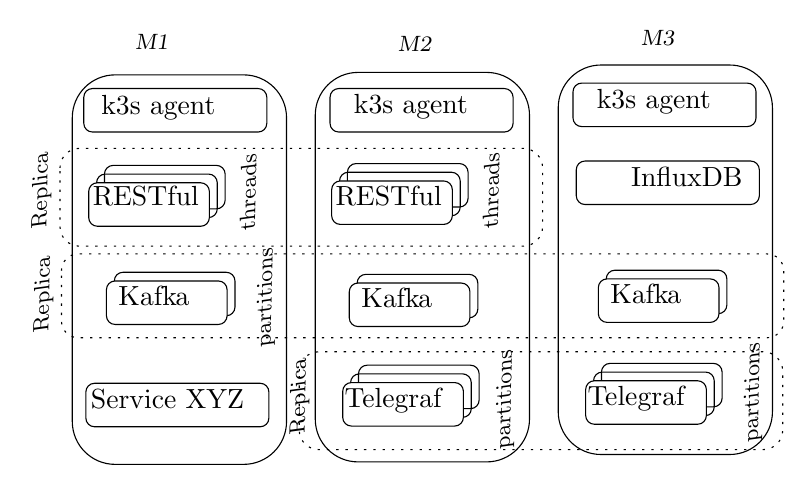
\begin{tikzpicture}[x=0.75pt,y=0.75pt,yscale=-1,xscale=1]
%uncomment if require: \path (0,300); %set diagram left start at 0, and has height of 300

%Rounded Rect [id:dp35697609560842714] 
\draw   (49.72,84.14) .. controls (49.72,81.82) and (51.6,79.95) .. (53.91,79.95) -- (103.67,79.95) .. controls (105.98,79.95) and (107.86,81.82) .. (107.86,84.14) -- (107.86,96.71) .. controls (107.86,99.02) and (105.98,100.9) .. (103.67,100.9) -- (53.91,100.9) .. controls (51.6,100.9) and (49.72,99.02) .. (49.72,96.71) -- cycle ;
%Rounded Rect [id:dp07253954089289416] 
\draw   (45.92,88.33) .. controls (45.92,86.01) and (47.8,84.14) .. (50.11,84.14) -- (99.87,84.14) .. controls (102.18,84.14) and (104.06,86.01) .. (104.06,88.33) -- (104.06,100.9) .. controls (104.06,103.21) and (102.18,105.09) .. (99.87,105.09) -- (50.11,105.09) .. controls (47.8,105.09) and (45.92,103.21) .. (45.92,100.9) -- cycle ;
%Rounded Rect [id:dp18871443500605878] 
\draw   (34.22,56.98) .. controls (34.22,45.58) and (43.46,36.34) .. (54.86,36.34) -- (116.79,36.34) .. controls (128.19,36.34) and (137.44,45.58) .. (137.44,56.98) -- (137.44,203.36) .. controls (137.44,214.76) and (128.19,224) .. (116.79,224) -- (54.86,224) .. controls (43.46,224) and (34.22,214.76) .. (34.22,203.36) -- cycle ;
%Rounded Rect [id:dp35402201539778266] 
\draw   (39.76,47.12) .. controls (39.76,44.81) and (41.63,42.93) .. (43.95,42.93) -- (123.75,42.93) .. controls (126.07,42.93) and (127.94,44.81) .. (127.94,47.12) -- (127.94,59.69) .. controls (127.94,62.01) and (126.07,63.88) .. (123.75,63.88) -- (43.95,63.88) .. controls (41.63,63.88) and (39.76,62.01) .. (39.76,59.69) -- cycle ;
%Rounded Rect [id:dp507370552804044] 
\draw  [fill={rgb, 255:red, 255; green, 255; blue, 255 }  ,fill opacity=1 ] (42.13,92.52) .. controls (42.13,90.2) and (44,88.33) .. (46.32,88.33) -- (96.07,88.33) .. controls (98.39,88.33) and (100.26,90.2) .. (100.26,92.52) -- (100.26,105.09) .. controls (100.26,107.4) and (98.39,109.28) .. (96.07,109.28) -- (46.32,109.28) .. controls (44,109.28) and (42.13,107.4) .. (42.13,105.09) -- cycle ;
%Rounded Rect [id:dp5704819195631831] 
\draw   (166.78,83.26) .. controls (166.78,80.95) and (168.66,79.07) .. (170.97,79.07) -- (220.72,79.07) .. controls (223.04,79.07) and (224.91,80.95) .. (224.91,83.26) -- (224.91,95.83) .. controls (224.91,98.15) and (223.04,100.02) .. (220.72,100.02) -- (170.97,100.02) .. controls (168.66,100.02) and (166.78,98.15) .. (166.78,95.83) -- cycle ;
%Rounded Rect [id:dp8793135885847785] 
\draw   (162.98,87.45) .. controls (162.98,85.14) and (164.86,83.26) .. (167.17,83.26) -- (216.93,83.26) .. controls (219.24,83.26) and (221.12,85.14) .. (221.12,87.45) -- (221.12,100.02) .. controls (221.12,102.34) and (219.24,104.21) .. (216.93,104.21) -- (167.17,104.21) .. controls (164.86,104.21) and (162.98,102.34) .. (162.98,100.02) -- cycle ;
%Rounded Rect [id:dp6083880622251631] 
\draw   (151.28,55.79) .. controls (151.28,44.39) and (160.52,35.15) .. (171.92,35.15) -- (233.85,35.15) .. controls (245.25,35.15) and (254.5,44.39) .. (254.5,55.79) -- (254.5,202.17) .. controls (254.5,213.57) and (245.25,222.81) .. (233.85,222.81) -- (171.92,222.81) .. controls (160.52,222.81) and (151.28,213.57) .. (151.28,202.17) -- cycle ;
%Rounded Rect [id:dp7318953389836701] 
\draw  [fill={rgb, 255:red, 255; green, 255; blue, 255 }  ,fill opacity=1 ] (159.19,91.64) .. controls (159.19,89.33) and (161.06,87.45) .. (163.38,87.45) -- (213.13,87.45) .. controls (215.45,87.45) and (217.32,89.33) .. (217.32,91.64) -- (217.32,104.21) .. controls (217.32,106.53) and (215.45,108.4) .. (213.13,108.4) -- (163.38,108.4) .. controls (161.06,108.4) and (159.19,106.53) .. (159.19,104.21) -- cycle ;
%Rounded Rect [id:dp6428078223562839] 
\draw  [dash pattern={on 0.84pt off 2.51pt}] (28.29,81.17) .. controls (28.29,75.96) and (32.51,71.74) .. (37.71,71.74) -- (251.4,71.74) .. controls (256.6,71.74) and (260.82,75.96) .. (260.82,81.17) -- (260.82,109.45) .. controls (260.82,114.66) and (256.6,118.88) .. (251.4,118.88) -- (37.71,118.88) .. controls (32.51,118.88) and (28.29,114.66) .. (28.29,109.45) -- cycle ;
%Rounded Rect [id:dp5401781780026212] 
\draw   (54.47,135.64) .. controls (54.47,133.32) and (56.34,131.45) .. (58.66,131.45) -- (108.41,131.45) .. controls (110.72,131.45) and (112.6,133.32) .. (112.6,135.64) -- (112.6,148.21) .. controls (112.6,150.52) and (110.72,152.4) .. (108.41,152.4) -- (58.66,152.4) .. controls (56.34,152.4) and (54.47,150.52) .. (54.47,148.21) -- cycle ;
%Rounded Rect [id:dp7933254515170439] 
\draw  [fill={rgb, 255:red, 255; green, 255; blue, 255 }  ,fill opacity=1 ] (50.67,139.83) .. controls (50.67,137.51) and (52.55,135.64) .. (54.86,135.64) -- (104.61,135.64) .. controls (106.93,135.64) and (108.8,137.51) .. (108.8,139.83) -- (108.8,152.4) .. controls (108.8,154.71) and (106.93,156.59) .. (104.61,156.59) -- (54.86,156.59) .. controls (52.55,156.59) and (50.67,154.71) .. (50.67,152.4) -- cycle ;
%Rounded Rect [id:dp26805012299713993] 
\draw   (158.4,47.12) .. controls (158.4,44.81) and (160.27,42.93) .. (162.59,42.93) -- (242.4,42.93) .. controls (244.71,42.93) and (246.59,44.81) .. (246.59,47.12) -- (246.59,59.69) .. controls (246.59,62.01) and (244.71,63.88) .. (242.4,63.88) -- (162.59,63.88) .. controls (160.27,63.88) and (158.4,62.01) .. (158.4,59.69) -- cycle ;
%Rounded Rect [id:dp18258581905382265] 
\draw   (268.34,52.23) .. controls (268.34,40.83) and (277.58,31.59) .. (288.98,31.59) -- (350.91,31.59) .. controls (362.31,31.59) and (371.55,40.83) .. (371.55,52.23) -- (371.55,198.61) .. controls (371.55,210.01) and (362.31,219.25) .. (350.91,219.25) -- (288.98,219.25) .. controls (277.58,219.25) and (268.34,210.01) .. (268.34,198.61) -- cycle ;
%Rounded Rect [id:dp9342611084348482] 
\draw   (275.46,44.5) .. controls (275.46,42.19) and (277.33,40.31) .. (279.65,40.31) -- (359.45,40.31) .. controls (361.77,40.31) and (363.64,42.19) .. (363.64,44.5) -- (363.64,57.07) .. controls (363.64,59.39) and (361.77,61.26) .. (359.45,61.26) -- (279.65,61.26) .. controls (277.33,61.26) and (275.46,59.39) .. (275.46,57.07) -- cycle ;
%Rounded Rect [id:dp640853487201022] 
\draw   (172.11,180.4) .. controls (172.11,178.09) and (173.98,176.21) .. (176.3,176.21) -- (226.05,176.21) .. controls (228.37,176.21) and (230.24,178.09) .. (230.24,180.4) -- (230.24,192.97) .. controls (230.24,195.29) and (228.37,197.16) .. (226.05,197.16) -- (176.3,197.16) .. controls (173.98,197.16) and (172.11,195.29) .. (172.11,192.97) -- cycle ;
%Rounded Rect [id:dp47472968878834354] 
\draw   (168.31,184.59) .. controls (168.31,182.28) and (170.19,180.4) .. (172.5,180.4) -- (222.26,180.4) .. controls (224.57,180.4) and (226.45,182.28) .. (226.45,184.59) -- (226.45,197.16) .. controls (226.45,199.48) and (224.57,201.35) .. (222.26,201.35) -- (172.5,201.35) .. controls (170.19,201.35) and (168.31,199.48) .. (168.31,197.16) -- cycle ;
%Rounded Rect [id:dp5083838851657617] 
\draw  [fill={rgb, 255:red, 255; green, 255; blue, 255 }  ,fill opacity=1 ] (164.51,188.78) .. controls (164.51,186.47) and (166.39,184.59) .. (168.7,184.59) -- (218.46,184.59) .. controls (220.77,184.59) and (222.65,186.47) .. (222.65,188.78) -- (222.65,201.35) .. controls (222.65,203.67) and (220.77,205.54) .. (218.46,205.54) -- (168.7,205.54) .. controls (166.39,205.54) and (164.51,203.67) .. (164.51,201.35) -- cycle ;
%Rounded Rect [id:dp30517511816997334] 
\draw   (289.17,179.53) .. controls (289.17,177.21) and (291.04,175.34) .. (293.36,175.34) -- (343.11,175.34) .. controls (345.42,175.34) and (347.3,177.21) .. (347.3,179.53) -- (347.3,192.1) .. controls (347.3,194.41) and (345.42,196.29) .. (343.11,196.29) -- (293.36,196.29) .. controls (291.04,196.29) and (289.17,194.41) .. (289.17,192.1) -- cycle ;
%Rounded Rect [id:dp42250294348135864] 
\draw   (285.37,183.72) .. controls (285.37,181.4) and (287.25,179.53) .. (289.56,179.53) -- (339.31,179.53) .. controls (341.63,179.53) and (343.5,181.4) .. (343.5,183.72) -- (343.5,196.29) .. controls (343.5,198.6) and (341.63,200.48) .. (339.31,200.48) -- (289.56,200.48) .. controls (287.25,200.48) and (285.37,198.6) .. (285.37,196.29) -- cycle ;
%Rounded Rect [id:dp04424150469326238] 
\draw  [fill={rgb, 255:red, 255; green, 255; blue, 255 }  ,fill opacity=1 ] (281.57,187.91) .. controls (281.57,185.59) and (283.45,183.72) .. (285.76,183.72) -- (335.52,183.72) .. controls (337.83,183.72) and (339.71,185.59) .. (339.71,187.91) -- (339.71,200.48) .. controls (339.71,202.79) and (337.83,204.67) .. (335.52,204.67) -- (285.76,204.67) .. controls (283.45,204.67) and (281.57,202.79) .. (281.57,200.48) -- cycle ;
%Rounded Rect [id:dp08404713866184521] 
\draw  [dash pattern={on 0.84pt off 2.51pt}] (143.55,179.18) .. controls (143.55,173.97) and (147.78,169.75) .. (152.98,169.75) -- (367.07,169.75) .. controls (372.28,169.75) and (376.5,173.97) .. (376.5,179.18) -- (376.5,207.46) .. controls (376.5,212.67) and (372.28,216.89) .. (367.07,216.89) -- (152.98,216.89) .. controls (147.78,216.89) and (143.55,212.67) .. (143.55,207.46) -- cycle ;
%Rounded Rect [id:dp42790792623498874] 
\draw   (277.04,82.04) .. controls (277.04,79.73) and (278.91,77.85) .. (281.23,77.85) -- (361.04,77.85) .. controls (363.35,77.85) and (365.23,79.73) .. (365.23,82.04) -- (365.23,94.61) .. controls (365.23,96.92) and (363.35,98.8) .. (361.04,98.8) -- (281.23,98.8) .. controls (278.91,98.8) and (277.04,96.92) .. (277.04,94.61) -- cycle ;
%Rounded Rect [id:dp6193243069663232] 
\draw   (171.47,136.64) .. controls (171.47,134.32) and (173.34,132.45) .. (175.66,132.45) -- (225.41,132.45) .. controls (227.72,132.45) and (229.6,134.32) .. (229.6,136.64) -- (229.6,149.21) .. controls (229.6,151.52) and (227.72,153.4) .. (225.41,153.4) -- (175.66,153.4) .. controls (173.34,153.4) and (171.47,151.52) .. (171.47,149.21) -- cycle ;
%Rounded Rect [id:dp14578003439060938] 
\draw  [fill={rgb, 255:red, 255; green, 255; blue, 255 }  ,fill opacity=1 ] (167.67,140.83) .. controls (167.67,138.51) and (169.55,136.64) .. (171.86,136.64) -- (221.61,136.64) .. controls (223.93,136.64) and (225.8,138.51) .. (225.8,140.83) -- (225.8,153.4) .. controls (225.8,155.71) and (223.93,157.59) .. (221.61,157.59) -- (171.86,157.59) .. controls (169.55,157.59) and (167.67,155.71) .. (167.67,153.4) -- cycle ;
%Rounded Rect [id:dp5296878196363403] 
\draw   (291.47,134.64) .. controls (291.47,132.32) and (293.34,130.45) .. (295.66,130.45) -- (345.41,130.45) .. controls (347.72,130.45) and (349.6,132.32) .. (349.6,134.64) -- (349.6,147.21) .. controls (349.6,149.52) and (347.72,151.4) .. (345.41,151.4) -- (295.66,151.4) .. controls (293.34,151.4) and (291.47,149.52) .. (291.47,147.21) -- cycle ;
%Rounded Rect [id:dp27455911002793476] 
\draw  [fill={rgb, 255:red, 255; green, 255; blue, 255 }  ,fill opacity=1 ] (287.67,138.83) .. controls (287.67,136.51) and (289.55,134.64) .. (291.86,134.64) -- (341.61,134.64) .. controls (343.93,134.64) and (345.8,136.51) .. (345.8,138.83) -- (345.8,151.4) .. controls (345.8,153.71) and (343.93,155.59) .. (341.61,155.59) -- (291.86,155.59) .. controls (289.55,155.59) and (287.67,153.71) .. (287.67,151.4) -- cycle ;
%Rounded Rect [id:dp26582997889434135] 
\draw  [dash pattern={on 0.84pt off 2.51pt}] (29,130.69) .. controls (29,126.23) and (32.62,122.61) .. (37.08,122.61) -- (368.92,122.61) .. controls (373.38,122.61) and (377,126.23) .. (377,130.69) -- (377,154.92) .. controls (377,159.38) and (373.38,163) .. (368.92,163) -- (37.08,163) .. controls (32.62,163) and (29,159.38) .. (29,154.92) -- cycle ;
%Rounded Rect [id:dp5354984118933027] 
\draw   (40.76,189.12) .. controls (40.76,186.81) and (42.63,184.93) .. (44.95,184.93) -- (124.75,184.93) .. controls (127.07,184.93) and (128.94,186.81) .. (128.94,189.12) -- (128.94,201.69) .. controls (128.94,204.01) and (127.07,205.88) .. (124.75,205.88) -- (44.95,205.88) .. controls (42.63,205.88) and (40.76,204.01) .. (40.76,201.69) -- cycle ;

% Text Node
\draw (63.28,15.61) node [anchor=north west][inner sep=0.75pt]  [font=\footnotesize,xslant=0.16] [align=left] {\begin{minipage}[lt]{14.056875000000002pt}\setlength\topsep{0pt}
\begin{center}
M1
\end{center}

\end{minipage}};
% Text Node
\draw (12.99,114.01) node [anchor=north west][inner sep=0.75pt]  [font=\footnotesize,rotate=-271.22,xslant=-0.16] [align=left] {\begin{minipage}[lt]{29.941250000000004pt}\setlength\topsep{0pt}
\begin{center}
Replica
\end{center}

\end{minipage}};
% Text Node
\draw (46.95,44.93) node [anchor=north west][inner sep=0.75pt]   [align=left] {k3s agent};
% Text Node
\draw (42.82,88.86) node [anchor=north west][inner sep=0.75pt]   [align=left] {RESTful};
% Text Node
\draw (113.44,115.01) node [anchor=north west][inner sep=0.75pt]  [font=\footnotesize,rotate=-271.22,xslant=-0.16] [align=left] {\begin{minipage}[lt]{29.941250000000004pt}\setlength\topsep{0pt}
\begin{center}
threads
\end{center}

\end{minipage}};
% Text Node
\draw (189.83,16.48) node [anchor=north west][inner sep=0.75pt]  [font=\footnotesize,xslant=0.16] [align=left] {\begin{minipage}[lt]{14.056875000000002pt}\setlength\topsep{0pt}
\begin{center}
M2
\end{center}

\end{minipage}};
% Text Node
\draw (230.5,114.14) node [anchor=north west][inner sep=0.75pt]  [font=\footnotesize,rotate=-271.22,xslant=-0.16] [align=left] {\begin{minipage}[lt]{29.941250000000004pt}\setlength\topsep{0pt}
\begin{center}
threads
\end{center}

\end{minipage}};
% Text Node
\draw (55.19,137) node [anchor=north west][inner sep=0.75pt]   [align=left] {Kafka};
% Text Node
\draw (115.79,170.45) node [anchor=north west][inner sep=0.75pt]  [font=\footnotesize,rotate=-271.22,xslant=-0.16] [align=left] {\begin{minipage}[lt]{35.838125000000005pt}\setlength\topsep{0pt}
\begin{center}
partitions
\end{center}

\end{minipage}};
% Text Node
\draw (168.64,44.47) node [anchor=north west][inner sep=0.75pt]   [align=left] {k3s agent};
% Text Node
\draw (306.89,13.87) node [anchor=north west][inner sep=0.75pt]  [font=\footnotesize,xslant=0.16] [align=left] {\begin{minipage}[lt]{14.056875000000002pt}\setlength\topsep{0pt}
\begin{center}
M3
\end{center}

\end{minipage}};
% Text Node
\draw (285.69,41.85) node [anchor=north west][inner sep=0.75pt]   [align=left] {k3s agent};
% Text Node
\draw (137.38,213.28) node [anchor=north west][inner sep=0.75pt]  [font=\footnotesize,rotate=-271.22,xslant=-0.16] [align=left] {\begin{minipage}[lt]{29.941250000000004pt}\setlength\topsep{0pt}
\begin{center}
Replica
\end{center}

\end{minipage}};
% Text Node
\draw (164.14,186.13) node [anchor=north west][inner sep=0.75pt]   [align=left] {Telegraf};
% Text Node
\draw (231.06,219.58) node [anchor=north west][inner sep=0.75pt]  [font=\footnotesize,rotate=-271.22,xslant=-0.16] [align=left] {\begin{minipage}[lt]{35.838125000000005pt}\setlength\topsep{0pt}
\begin{center}
partitions
\end{center}

\end{minipage}};
% Text Node
\draw (281.2,185.26) node [anchor=north west][inner sep=0.75pt]   [align=left] {Telegraf};
% Text Node
\draw (350.49,216.08) node [anchor=north west][inner sep=0.75pt]  [font=\footnotesize,rotate=-271.22,xslant=-0.16] [align=left] {\begin{minipage}[lt]{35.838125000000005pt}\setlength\topsep{0pt}
\begin{center}
partitions
\end{center}

\end{minipage}};
% Text Node
\draw (302.17,79.39) node [anchor=north west][inner sep=0.75pt]   [align=left] {InfluxDB};
% Text Node
\draw (159.82,88.86) node [anchor=north west][inner sep=0.75pt]   [align=left] {RESTful};
% Text Node
\draw (172.19,138) node [anchor=north west][inner sep=0.75pt]   [align=left] {Kafka};
% Text Node
\draw (292.19,136) node [anchor=north west][inner sep=0.75pt]   [align=left] {Kafka};
% Text Node
\draw (13.99,164.01) node [anchor=north west][inner sep=0.75pt]  [font=\footnotesize,rotate=-271.22,xslant=-0.16] [align=left] {\begin{minipage}[lt]{29.941250000000004pt}\setlength\topsep{0pt}
\begin{center}
Replica
\end{center}

\end{minipage}};
% Text Node
\draw (41.95,186.93) node [anchor=north west][inner sep=0.75pt]   [align=left] {Service XYZ};


\end{tikzpicture}


    \caption{A topological view of how, with respect to the 3 servers in the ICE lab, how the various services are instantiated. For example, for Kafka, having an instance on all 3 servers, the k3s agent will act as a load balancer to distribute the traffic among the various servers. (M1, M2 and M3).}
    \label{TopologyExample}
\end{figure}

    Figure ~\ref{TopologyExample} shows at the topological level how k3s could distribute the various pods and replicas among the three servers during the test execution.
In fact, the tests were run starting with a distribution of pods without replicas and multithreads, and later augmenting and combining the parameters.

Two types of tests were then identified: the first type, using HIVE in a static manner, to test given the specific configuration of HIVE how the architecture response behaves with respect to the configuration of the pods.
The second test, instead, was to execute HIVE dynamically, in order to perform a stress test of longer duration and with a higher number of requests once the configuration of the architecture to be tested was identified.

The purpose of the test, was to be able to find the load limit that the REST APIs can handle, but not only: in fact, another goal is to find out how is possible to reduce the delay between the REST APIs and the InfluxDB database, exploiting replication and topic management between Kafka and Telegraf.
\\

The test run was done in one day, so targeted testing had to be done based on HIVE and architecture configurations.
Table ~\ref{tab:results} shows the results as number of requests per second handled by the RESTful server by the HIVE configuration and architecture parameters variance.

\begin{table*}[!ht]
\centering
\resizebox{\textwidth}{!}{
\begin{tabular}{c||ccc|ccc||ccc||c||ccc||ccccc||}
\hline
Session&
\multicolumn{6}{c||}{HIVE} & \multicolumn{3}{c||}{REST API} & \multicolumn{1}{c||}{Kafka}&
\multicolumn{3}{c||}{Telegraf} 
&\multicolumn{5}{c||}{Results} \\
Number & 
wrk & Max & Max & Amount & Conn & Pip & Replicas & wrk & CPU [\%] & Partitions & Flush  & Interval & Replicas & Tot & Avg  & Db Delay & K Delay & R Delay \\
&&Conn&Pip&&&&&&Usage&&[s]&[s]&&Req&Req/s&[s]&[s]&[s]\\
\hline
\hline
1  & 1 & -   & -  & 10   & 1  & 1  & 1 & 1 & 10   & 1 & 10 & 5 & 1 & 100  & 10    & 0,81 & -    & 0,08\\
2  & 1 & -   & -  & 10   & 1  & 1  & 1 & 1 & 10   & 1 & 10 & 5 & 1 & 100  & 10    & 0,67 & 0,92 & 0,08\\
3  & 1 & -   & -  & 500  & 1  & 1  & 1 & 1 & 30   & 1 & 10 & 5 & 1 & 5k   & 500   & 12,1 & -& 0,01\\
4  & 1 & -   & -  & 500  & 1  & 1  & 1 & 1 & 30   & 1 & 10 & 5 & 1 & 5k   & 500   & 14,1 & 0,10 & 0,07\\
5  & 1 & -   & -  & 500  & 2  & 2  & 1 & 1 & 40   & 1 & 10 & 5 & 1 & 5k   & 500   & 21,3 & 0,10& 0,06\\
6  & 1 & -   & -  & 1500 & 1  & 1  & 1 & 1 & 40   & 1 & 10 & 5 & 1 & 15k  & 1263  & 46,3 & 0,86 & 0,07\\
7  & 1 & -   & -  & 1000 & 1  & 1  & 1 & 1 & 40   & 1 & 10 & 5 & 1 & 10k  & 1000  & 35,0 & 0,88 & 0,71\\
8  & 1 & -   & -  & 1200 & 2  & 1  & 1 & 1 & 40   & 1 & 10 & 5 & 1 & 12k  & 1194  & 46,2 & 0,78 & 3,34\\
9  & 1 & -   & -  & 1200 & 32 & 8  & 1 & 1 & 100  & 1 & 5  & 1 & 1 & 71k  & 7000  & -    & - & 3,34\\
10 & 1 & -   & -  & 1200 & 32 & 8   & 1 & 1 & 100 & 1 & 5  & 1 & 1 & 71k  & 7000  & 10,0 & 0,86& 3,30\\
11 & 1 & -   & -  & 1000 & 32 & 24  & 1 & 1 & 100 & 1 & 5  & 1 & 1 & 80k  & 7424  & 11,0 & 0,95& 3,67\\
12 & 1 & -   & -  & 2000 & 32 & 24  & 1 & 1 & 100 & 1 & 5  & 1 & 1 & 83k  & 7511  & 10,0 & 0,96& 3,67\\
13 & 1 & -   & -  & 2000 & 32 & 24  & 1 & 2 & 200 & 1 & 5  & 1 & 1 & 120k & 12000 & 20,0 & 0,92& 3,22\\
14 & 1 & -   & -  & 2000 & 32 & 24  & 1 & 2 & 200 & 1 & 1  & 1 & 1 & 125k & 12000 & 5,0  & 2,99& 3,20\\
15 & 1 & -   & -  & 1000 & 16 & 16  & 1 & 2 & 200 & 1 & 1  & 1 & 1 & 126k & 12000 & 4,0  & 1,48& 3,20\\
16 & 4 & -   & -  & 1000 & 16 & 16  & 1 & 2 & 200 & 1 & 1  & 1 & 1 & 135k & 14000 & 4,2  & -& 3,31\\
17 & 1 & 100 & 50 & -    & -  & -   & 1 & 2 & 200 & 1 & 1  & 1 & 1 & 160k & 15000 & -    & 1,50 & 3,52\\
18 & 4 & -   & -  & 2000 & 32 & 24  & 1 & 4 & 400 & 1 & 1  & 1 & 1 & 247k & 23000 & 11,2 & 3,99& 3,49\\
19 & 4 & 100 & 50 & -    & -  & -   & 1 & 4 & 400 & 1 & 1  & 1 & 1 & 261k & 30000 & -    & -& -\\
20 & 4 & -   & -  & 2000 & 32 & 24  & 1 & 4 & 400 & 1 & 1  & 1 & 3 & 270k & 50000 & 40,8 & 4,83 & 3,59\\
21 & 4 & -   & -  & 1000 & 1  & 1   & 1 & 4 & 400 & 1 & 1  & 1 & 3 & 42k  & 4000  & -    & 0,66 & 0,019\\
22 & 4 & -   & -  & 1000 & 1  & 1   & 1 & 4 & 400 & 3 & 1  & 1 & 3 & 42k  & 4000  & 0,55 & 0,69& 0,015\\
23 & 4 & -   & -  & 2000 & 32 & 24  & 1 & 4 & 400 & 3 & 1  & 1 & 3 & 250k & 25000 & 13,5 & 5,58& 0,017\\
24 & 4 & -   & -  & 2000 & 16 & 8   & 1 & 4 & 400 & 3 & 1  & 1 & 3 & 223k & 20000 & 0,76 & 0,35& 3,30\\
25 & 4 & -   & -  & 2000 & 32 & 16  & 4 & 4 & 250 & 3 & 1  & 1 & 3 & 300k & 30000 & 3,96 & 6,52& 3,54\\
26 & 4 & -   & -  & 2048 & 64 & 16  & 4 & 4 & 350 & 3 & 1  & 1 & 3 & 417k & 40000 & 6,23 & 10,92& 3,26\\
27 & 4 & -   & -  & 4096 & 64 & 16  & 4 & 4 & 400 & 3 & 1  & 1 & 3 & 482k & 48000 & 6,71 & 15,21& 3,17\\
28 & 4 & 100 & 50 & -    & -  & -   & 4 & 4 & 400 & 3 & 1  & 1 & 3 & 594k & 56000 & -    & -    & -\\

\end{tabular}}
% \vspace{-0.3cm}
\caption{The table shows the configuration of the k3s cluster (REST API, Kafka and Telegraf columns), the configuration of the HIVE tool (HIVE column) and the results obtained (Results column).}\label{tab:results}
\vspace{-0.5cm}
\end{table*}

\section{Results}
The table ~\ref{tab:results} shows the tests carried out (about 28 in total) with the relative performances obtained.
All tests are for a maximum duration of 10 seconds in both static and dynamic HIVE mode. The columns \textit{HIVE.wrk}, \textit{HIVE.maxConn} and \textit{HIVE.maxPip} refer to the parameters for dynamic execution of the HIVE tool. The remaining 3 columns instead refer to a static execution. It can be noticed in fact that they are mutually exclusive.

One thing that should be noted is that the estimate of the delay from HIVE to the Kafka client connected directly to the broker, is not precise (column \textit{K Delay}): the client has been written in Nodejs language, using only single-thread execution. It has been seen that during testing that the core used was always at 100\%, indicating that in all likelihood the data would be queued creating an additional delay. 
It should be noted, however, that in all tests where the machine running the Kafka client subscriber was not especially under stress, the calculated delay was below one second, indicating that the Kafka broker had no traffic flow problems.

Regarding the delay from HIVE and InfluxDB, however, you must take into account that the data represented in the \textit{Db Delay} column, has a delay due to the publishing of the data of the Kafka broker and Telegraf (note the column values of \textit{Telegraf.push} and \textit{Telegraf.interval}): if there is a flush of the data every \textit{10s}, it is normal that there is a delay of \textit{+10s} compared to the normal communication delay.

Another piece of information, but not less important, is the delay generated by HIVE to the REST API. This is the first delay that the architecture encounters and it is added to the one obtained later by the Kafka broker and the actual writing to InfluxDB. This value is reported in the \textit{R Delay} column.

\paragraph{Test 1-2}Tests 1 and 2 are really low load: the tool generate 10 requests per second (for a total of about 100 connections handled in 10 seconds), to verify that all services are up and ready within the architecture.
\paragraph{Test 3-8}The tests then continued with number 3 to 5 increasing the number of connections per second up to 500, while, from test 6 to 8 the number of request, the number of concurrent connections and the size of the HTTP pipelining factor was increased. With the configuration of test 8, 12k total requests were reached in \textit{10s}, but shows that an average delay (\textit{Db Delay}) quite high. 
\paragraph{Test 9-12}With test 9 through 23, is lowered the \textit{flush} and \textit{interval} values of Telegraf, increasing the number of requests/second to be satisfied by double. Specifically, with test 12, 83k total requests (7,5k/s on average) were reached. A great result knowing that the REST APIs are single threaded on a single core, and the architecture still all with a single replica and worker.
\paragraph{Test 13}
In test 13 the REST APIs were deployed with 2 workers to handle the load of requests. It is possible see how the total went up to 120k. This value starts to give us some insight into how linearly the load can scale when scaling vertically on the architecture.

\paragraph{Test 14-16}
In tests 14, 15, and 16 is tried to increase the number of requests to be suffused but it is noticed that the limit reached was around 130k total requests, making us realize that the REST APIs could handle at 100\% CPU usage around 70k total requests per core (7k req/s).

\paragraph{Test 17}
In test 17, was done a stress test with HIVE in dynamic mode, and is possible to notice that without having errors, varying the configurations of request generation, the 7,5k req/s was not exceeding, confirming the maximum load on average manageable by each core dedicated to the REST API.

\paragraph{Test 22-27}
From test 22 to 24 REST APIs were deployed to more cores, but also increased Kafka partitions and Telegraf replicas.
In tests 25, 26, and 27, it was scaled the REST APIs horizontally as well, resulting in about 482k satisfied requests (for an equal of about 48k requests per second). A very good value knowing that all the data arrived to the DB and there were no response errors from the REST API: it means that despite the load, they could be pushed a bit more before starting to fail to handle incoming requests.

\paragraph{Test 28}
Test 28 was performed in dynamic HIVE mode and was the last test performed on the test day. As you can see from the table ~\ref{tab:results}, but also from the Figure\ref{fig:graph01} you can see that with varying configurations the maximum load of 594k total requests (56k req/s) was obtained with a factor of 100 of concurrent requests and 50 as a factor of HTTP pipelining.
Also, thanks to the delay Figure (~\ref{fig:graph02}), is visible that the best handling is with 50 pipelining factor and 20 concurrent connections without having errors (~\ref{fig:graph03}).

\begin{figure}[ht]
\centering
\includegraphics[width=0.45\textwidth, page={5}]{0_req.png}
\vspace{-0.25cm}
\caption{Graph showing how the number of PUT req/s varies with respect to the number of concurrent connections and the HTTP pipelining factor. The maximum peak is 56k req/s. Each test had a duration of 10 seconds.}
\label{fig:graph01}
\vspace{-0.25cm}
\end{figure}

\begin{figure}[ht]
\centering
\includegraphics[width=0.45\textwidth, page={5}]{0_avg.png}
\vspace{-0.25cm}
\caption{Graph showing how the number of ms of latency req/s varies with respect to the number of concurrent connections and the HTTP pipelining factor in the communication between HIVE and the RESTful server. Each test had a duration of 10 seconds.}
\label{fig:graph02}
\vspace{-0.25cm}
\end{figure}


\begin{figure}[ht]
\centering
\includegraphics[width=0.45\textwidth, page={5}]{0_err.png}
\vspace{-0.25cm}
\caption{Graph showing how the number of errors varies with respect to the number of concurrent connections and the HTTP pipelining factor in the communication between HIVE and the RESTful server. Each test had a duration of 10 seconds.}
\label{fig:graph03}
\vspace{-0.25cm}
\end{figure}




\begin{figure}[!bht]
\centering
\includegraphics[width=0.45\textwidth, page={6}]{1_req.png}
\vspace{-0.25cm}
\caption{Graph showing how the number of GET req/s varies with respect to the number of concurrent connections and the HTTP pipelining factor. The maximum peak is 120k req/s. Each test had a duration of 10 seconds.}
\label{fig:get1}
\vspace{-0.25cm}
\end{figure}


\begin{figure}[!bht]
\centering
\includegraphics[width=0.45\textwidth, page={6}]{1_avg.png}
\vspace{-0.25cm}
\caption{Graph showing how the number of ms of latency req/s varies with respect to the number of concurrent connections and the HTTP pipelining factor in the communication between HIVE and the RESTful server. Each test had a duration of 10 seconds.}
\label{fig:get2}
\vspace{-0.25cm}
\end{figure}

\paragraph{What about GET requests?}

While is not identify a real-world scenario in which the REST APIs would be queried frequently to move the architecture on a critical point, just for information, a test to see how many GET requests the server could handle it has been carried out the same. Note that all the tests run so far were PUTs with a payload. A total of $1,2*10^6$ requests were reached in \textit{10s}. In Figure ~\ref{fig:get1} is reported the variance of the requests average and in Figure ~\ref{fig:get2} the variance of the delay.

\section{Conclusion}
It has been demonstrated how the RESTful server can handle 56k requests per second with 100 concurrent connections.

Is possible to see that the request load is variable with respect to the available hardware resources: in fact, the increase of requests per second is linear with respect to the number of cores available to the RESTful server.

Thanks to this test, an alternative to the OPC-UA protocol is proposed to communicate with the data collection architecture of the ICE lab, but it is also demonstrated that the bottleneck is actually the RESTful server. The Kafka broker, Telegraf and InfluxDB, handled without difficulty the large load of requests, indicating the fact that the architecture could probably handle a much larger amount of data than we achieved in these tests.



\section{Future Works}
Nodejs configuration with Fastify may not the best. According to the github ~\cite{gitweb} performance document, the RESTful server in java might be the one that can handle the largest number of requests. Future works could undoubtedly be to try a java-based architecture.
Further analysis can be done on how Kafka and Telegraf handles data flushing, and how pods can be more efficiently balanced within the architecture.
As far as the request generator (HIVE) is concerned, it is possible to find (or develop) new alternatives that generate even more requests.

\section{acknowledgements}
I would like to thanks Professor D. Carra for the opportunity given to me to create an application in the ICE lab, M. Panato and C. Tadiello for supporting me in the development and execution of the tests within the ICE Lab.
All the work done is available and documented on the gitlab repository of ICE lab.

\bibliography{biblio}
\bibliographystyle{IEEEtran}
    
    

\end{document}
